% ============================================================
% HSBI Beamer — ISLP Lecture Series (English) — IMPROVED EDITION
% Chapter 3: Linear Regression
%
% Pedagogical revision: each concept is introduced with motivation,
% intuition, formal definition, worked example, interpretation, and
% practical relevance. Slide titles are descriptive. Formulas are
% explained symbol-by-symbol with concrete worked numbers.
% ============================================================

\documentclass[aspectratio=169,11pt]{beamer}

\usepackage[utf8]{inputenc}
\usepackage[T1]{fontenc}
\usepackage[english]{babel}
\usepackage{graphicx}
\usepackage{booktabs}
\usepackage{amsmath,amssymb,amsfonts}
\usepackage{mathtools}
\usepackage{hyperref}
\usepackage{xcolor}
\usepackage{verbatim}
\usepackage{alltt}
\usepackage{tikz}
\usetikzlibrary{calc,arrows.meta,positioning,decorations.pathreplacing,shapes}
\usepackage{tcolorbox}
\tcbuselibrary{skins}

\usetheme{Madrid}
\usecolortheme{default}
\setbeamertemplate{navigation symbols}{}
\setbeamertemplate{footline}[frame number]
\setbeamertemplate{blocks}[rounded][shadow=false]
\setbeamertemplate{headline}{%
  \leavevmode\hbox{%
    \begin{beamercolorbox}[wd=\paperwidth,ht=2.2ex,dp=0.9ex]{section in head/foot}%
      {\fontsize{4.6}{5.2}\selectfont%
       \insertsectionnavigationhorizontal{\paperwidth}{}{\hskip0pt plus1filll}}%
    \end{beamercolorbox}}%
}
\setbeamerfont{section in head/foot}{size=\tiny}
\setbeamerfont{palette primary}{size=\tiny}
\setbeamerfont{palette tertiary}{size=\tiny}
\setbeamerfont{section in toc}{size=\footnotesize}

\usepackage{listings}
\definecolor{pyKw}{RGB}{0,0,180}
\definecolor{pyStr}{RGB}{20,120,40}
\definecolor{pyCom}{RGB}{120,120,120}
\definecolor{accent}{RGB}{38,70,140}
\definecolor{accentLight}{RGB}{220,228,245}
\lstdefinestyle{Pystyle}{
  language=Python, basicstyle=\ttfamily\footnotesize\linespread{0.9}\selectfont,
  keywordstyle=\color{pyKw}\bfseries, commentstyle=\color{pyCom}\itshape,
  stringstyle=\color{pyStr}, showstringspaces=false, upquote=true,
  columns=fullflexible, breaklines=true, literate={~}{{$\sim$}}1
}
\lstset{style=Pystyle}

\AtBeginSection[]{%
  \begin{frame}{Outline}
  \begin{columns}[t]
    \begin{column}{0.5\textwidth}
      \tableofcontents[currentsection,sectionstyle=show/shaded,subsectionstyle=show/show/hide,sections={1-4}]
    \end{column}
    \begin{column}{0.5\textwidth}
      \tableofcontents[currentsection,sectionstyle=show/shaded,subsectionstyle=show/show/hide,sections={5-8}]
    \end{column}
  \end{columns}
  \end{frame}
}

\newcommand{\islpsource}[1]{%
  \vfill
  \hfill{\tiny\itshape\color{gray}Source: #1 \textemdash{} ISLP, James et al.\ (2023).}\par
}

% Custom callout box: green left bar, light green fill --- for "intuition / takeaway"
\newtcolorbox{takeaway}[1][Takeaway]{%
  enhanced, colback=green!4, colframe=green!50!black,
  boxrule=0pt, leftrule=2.5pt, arc=2pt, fonttitle=\bfseries,
  title=#1, left=2mm, right=2mm, top=1mm, bottom=1mm
}

% Custom callout box: orange/yellow --- for "worked example with numbers"
\newtcolorbox{numexample}[1][Worked example]{%
  enhanced, colback=orange!4, colframe=orange!70!black,
  boxrule=0pt, leftrule=2.5pt, arc=2pt, fonttitle=\bfseries,
  title=#1, left=2mm, right=2mm, top=1mm, bottom=1mm
}

% Custom callout box: light blue --- for "how to read this formula"
\newtcolorbox{readme}[1][How to read this]{%
  enhanced, colback=blue!4, colframe=accent,
  boxrule=0pt, leftrule=2.5pt, arc=2pt, fonttitle=\bfseries,
  title=#1, left=2mm, right=2mm, top=1mm, bottom=1mm
}

\title{Quantitative Research Methods}
\subtitle{Chapter 3: Linear Regression}
\author{Prof.\ Dr.\ Christoph Weisser}
\institute{HSBI}
\date{Summer Semester 2026}

\graphicspath{{images/}}

% Exercise / solution callout boxes (in-deck exercises)
\newtcolorbox{exercise}[1][Exercise]{enhanced, fontupper=\footnotesize, colback=purple!4, colframe=purple!55!black, boxrule=0pt, leftrule=2.5pt, arc=2pt, fonttitle=\bfseries, title=#1, left=2mm, right=2mm, top=1mm, bottom=1mm}
\newtcolorbox{solutionbox}[1][Solution]{enhanced, fontupper=\footnotesize, colback=teal!5, colframe=teal!55!black, boxrule=0pt, leftrule=2.5pt, arc=2pt, fonttitle=\bfseries, title=#1, left=2mm, right=2mm, top=1mm, bottom=1mm}

% Reclaim ~2pt of body height (custom nav headline makes full slides tip over by ~1.83pt)
\addtobeamertemplate{frametitle}{}{\vspace{-2pt}}

% Extended (integrative ~15 min) exercise callout box --- violet, distinct from short exercises
\newtcolorbox{longexercise}[1][Extended exercise (15 min)]{enhanced, fontupper=\footnotesize, colback=violet!6, colframe=violet!55!black, boxrule=0pt, leftrule=3pt, arc=2pt, fonttitle=\bfseries, title=#1, left=2mm, right=2mm, top=1mm, bottom=1mm}

\newtcolorbox{labnote}[1][Run this live in the lab notebook]{enhanced, fontupper=\footnotesize, colback=cyan!7, colframe=cyan!45!black, boxrule=0pt, leftrule=3pt, arc=2pt, fonttitle=\bfseries, title=#1, left=2mm, right=2mm, top=1mm, bottom=1mm}

\begin{document}

\begin{frame}[plain]
  \titlepage
\end{frame}

\begin{frame}{The course at a glance}
  \footnotesize
  \begin{center}
  \begin{tabular}{@{}c r l@{}}
    & \textbf{Lecture} & \textbf{Topic}\\
    \midrule
     & 1 & Ch.\ 1 + 2 --- Introduction; what is statistical learning \\
     & 2 & Ch.\ 2 --- Accuracy, bias--variance, Bayes classifier, KNN \\
    $\blacktriangleright$ & \textbf{3--4} & \textbf{Ch.\ 3 --- Linear regression (estimation, inference, diagnostics)} \\
     & 5--6 & Ch.\ 4 --- Classification (logistic, LDA/QDA, naive Bayes, ROC) \\
     & 7 & Ch.\ 5 --- Resampling (validation, CV, bootstrap) \\
     & 8 & Ch.\ 6 --- Model selection and regularisation (ridge, lasso) \\
     & 9 & Ch.\ 7 --- Moving beyond linearity (splines, GAMs) \\
     & 10 & Ch.\ 8 --- Tree-based methods (trees, forests, boosting) \\
     & 11 & Ch.\ 10 --- Deep learning (MLPs, CNNs, training) \\
     & 12 & Ch.\ 13 --- Multiple testing (FWER, FDR) \\
  \end{tabular}
  \end{center}
  \vspace{2pt}
  {\scriptsize Twelve sessions of 180 minutes. $\blacktriangleright$ marks today's chapter. Short exercises every $\sim$20 min; extended exercises every $\sim$45 min; each chapter has a companion lab notebook.}
\end{frame}



\begin{frame}{Contents}\footnotesize
  \tableofcontents[hideallsubsections]
\end{frame}

\begin{frame}{Notation in this chapter}
  \footnotesize
  \begin{center}
  \begin{tabular}{@{}ll@{}}
    \toprule
    \textbf{Symbol} & \textbf{Meaning} \\
    \midrule
    $\beta_0,\ \beta_1$ & Population intercept and slope; hats ($\hat\beta_0,\hat\beta_1$) mark least-squares estimates. \\
    $e_i = y_i - \hat y_i$ & Residual: observed minus fitted value for observation $i$. \\
    $\mathrm{RSS}=\sum_i e_i^2$ & Residual sum of squares --- the quantity least squares minimises. \\
    $\sigma$,\ $\mathrm{RSE}$ & Error standard deviation; estimated by $\mathrm{RSE}=\sqrt{\mathrm{RSS}/(n-2)}$. \\
    $\mathrm{SE}(\hat\beta_1)$ & Standard error: sample-to-sample variability of the slope estimate. \\
    $t=\hat\beta_1/\mathrm{SE}(\hat\beta_1)$ & $t$-statistic for testing $H_0\colon \beta_1 = 0$. \\
    $R^2 = 1-\mathrm{RSS}/\mathrm{TSS}$ & Fraction of variance explained; $\mathrm{TSS}=\sum_i(y_i-\bar y)^2$. \\
    $F$ & $F$-statistic: tests all slopes at once, $H_0\colon\beta_1=\dots=\beta_p=0$. \\
    $h_{ii}$ & Leverage of observation $i$: how unusual its predictor values are. \\
    $\mathrm{VIF}(\hat\beta_j)$ & Variance inflation factor: collinearity of $X_j$ with the other predictors. \\
    \bottomrule
  \end{tabular}
  \end{center}
  \vspace{2pt}
  {\scriptsize Symbols are listed in order of first appearance; each is defined in full on the slide where it first occurs.}
\end{frame}

\begin{frame}{Sources and references}
  \begin{block}{Primary textbook}
    James, G., Witten, D., Hastie, T., Tibshirani, R., \& Taylor, J.\ (2023).\\
    \emph{An Introduction to Statistical Learning, with Applications in
    Python.} Springer. \texttt{www.statlearning.com}.
  \end{block}
  \begin{block}{About these slides}
    Compared with the standard chapter deck, every concept is now
    introduced with explicit \emph{motivation}, \emph{intuition},
    \emph{formal definition}, \emph{worked example}, and \emph{practical
    interpretation}. Slide titles are descriptive; formulas are
    explained symbol-by-symbol.
  \end{block}
\end{frame}

\begin{frame}{Learning objectives for this chapter}
  By the end of this chapter you will be able to:
  \begin{itemize}
    \item \textbf{Estimate} simple and multiple linear regression
          coefficients by ordinary least squares, and interpret each
          coefficient correctly --- including the ``holding others
          fixed'' clause.
    \item \textbf{Test} the relevant hypotheses ($t$ for one
          coefficient, $F$ for several at once) and \textbf{construct}
          confidence intervals.
    \item \textbf{Distinguish} a confidence interval for the regression
          line from a prediction interval for an individual outcome.
    \item \textbf{Diagnose} the four classical regression problems ---
          nonlinearity, heteroscedasticity, outliers / leverage,
          collinearity --- and apply the standard remedies.
    \item \textbf{Encode} qualitative predictors and \textbf{add}
          interaction terms following the hierarchy principle.
    \item \textbf{Compare} linear regression with nonparametric
          alternatives (KNN regression).
  \end{itemize}
\end{frame}


\begin{frame}{Roadmap of this chapter}
  \begin{takeaway}[The path through linear regression]
    \begin{enumerate}
      \item Motivation: the Advertising problem.
      \item Simple linear regression: model, estimation, inference.
      \item Multiple linear regression: confounding, the four key questions.
      \item Extensions: dummies, interactions, polynomials.
      \item Diagnostics: nonlinearity, heteroscedasticity, leverage,
            collinearity.
      \item Comparison with KNN regression.
    \end{enumerate}
  \end{takeaway}
\end{frame}

% ============================================================
\section{Why this chapter matters}
% ============================================================

\begin{frame}{Why is linear regression still in every textbook?}
  Linear regression was published in 1805. Why are we still teaching it
  in 2026?
  \begin{takeaway}[Three reasons]
    \begin{enumerate}
      \item It is the \emph{most widely deployed} statistical model in
            industry --- finance, medicine, marketing, public policy.
      \item It comes with a \emph{complete inference toolkit} (standard
            errors, $p$-values, prediction intervals).
      \item It is the \emph{benchmark} against which fancier methods
            (random forests, neural nets) are routinely compared. Many
            of those fancier methods only barely beat linear
            regression on real data.
    \end{enumerate}
  \end{takeaway}
  This chapter gives you everything you need to fit, interpret,
  diagnose, and defend a linear regression in any setting.
\end{frame}

\begin{frame}{Concrete client problem: the Advertising data}
  \begin{columns}[T]
    \begin{column}{0.55\textwidth}
      \begin{block}{The brief}
        A marketing client has spent budget on TV, radio, and newspaper
        advertising in 200 different markets. Sales are recorded per
        market. The client asks:
        \begin{quote}
          \emph{``Where should I put next year's budget?''}
        \end{quote}
      \end{block}
      \begin{block}{Variables}
        \begin{itemize}
          \item Response: \texttt{sales} (units, in 1{,}000s).
          \item Predictors: \texttt{TV}, \texttt{radio},
                \texttt{newspaper} budgets (in \$1{,}000).
          \item $n = 200$ markets.
        \end{itemize}
      \end{block}
    \end{column}
    \begin{column}{0.42\textwidth}
      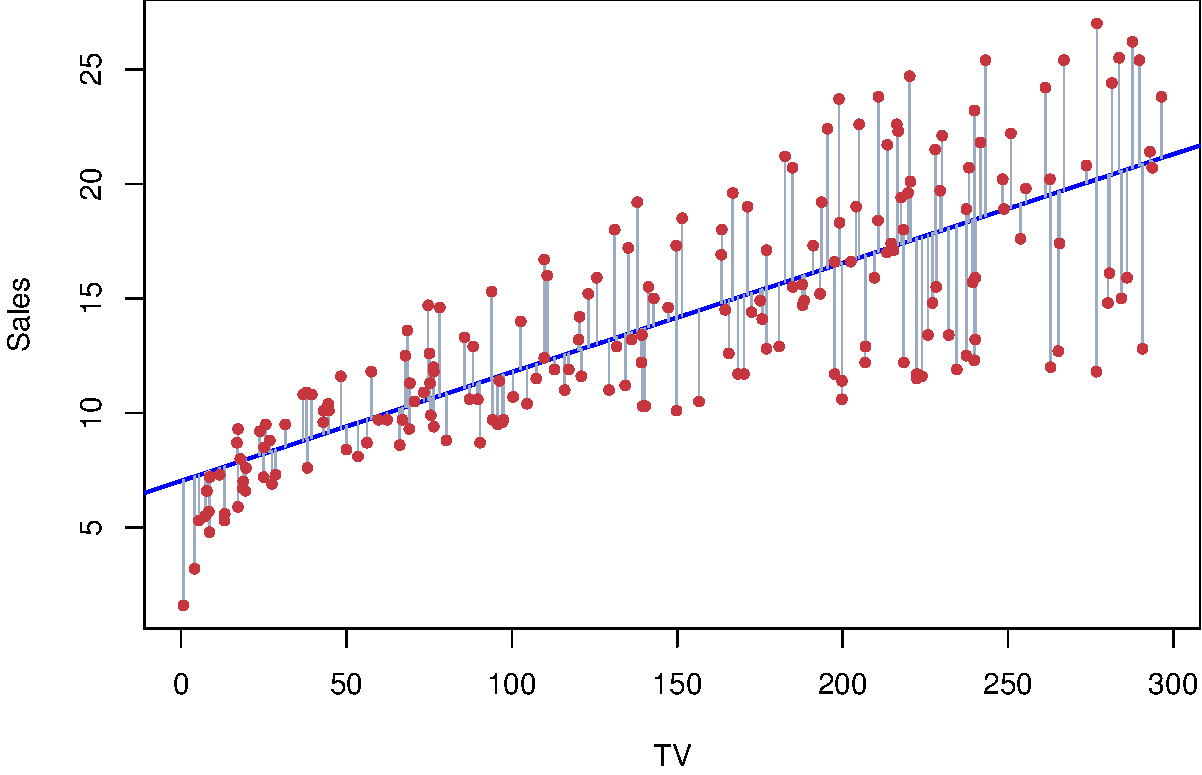
\includegraphics[width=\textwidth,height=0.65\textheight,keepaspectratio]{3_1.pdf}
    \end{column}
  \end{columns}
  \islpsource{Figure 3.1}
\end{frame}

\begin{frame}{The raw data: sales against each medium}
  \begin{center}
    
\includegraphics[width=0.95\textwidth,height=0.6\textheight,keepaspectratio]{ch03_three_predictors.png}
  \end{center}
  \begin{takeaway}[First look]
    Sales rise clearly with TV and radio spend; the newspaper trend is
    weak. Each panel is a \emph{simple} regression --- the multiple
    regression later will revise these single-predictor slopes.
  \end{takeaway}
\end{frame}

\begin{frame}{Seven concrete questions linear regression can answer}
  Before we look at any formulas, notice that one data set lets us
  answer many \emph{different} questions:
  \begin{enumerate}
    \item Is there \emph{any} relationship between advertising and
          sales?
    \item How \emph{strong} is that relationship?
    \item Which media \emph{contribute} --- and which do not?
    \item How \emph{precise} are our estimated effects?
    \item How well can we \emph{predict} next quarter's sales?
    \item Is the relationship between spend and sales \emph{linear}?
    \item Is there \emph{synergy} (interaction) among the media?
  \end{enumerate}
  Each question maps to a specific tool we will develop in this
  chapter. Keep them in mind as we go.
\end{frame}

\begin{frame}{What linear regression delivers --- and what it does not}
  \begin{columns}[T]
    \begin{column}{0.48\textwidth}
      \begin{block}{What you get}
        \begin{itemize}
          \item Coefficients you can interpret.
          \item Standard errors and tests.
          \item Confidence and prediction intervals.
          \item Diagnostic plots.
        \end{itemize}
      \end{block}
    \end{column}
    \begin{column}{0.48\textwidth}
      \begin{alertblock}{What you do not automatically get}
        \begin{itemize}
          \item \emph{Causality.} A coefficient is an association, not
                a cause.
          \item \emph{Validity outside the data range.} Extrapolation is
                always risky.
          \item \emph{Robustness to gross outliers.} Leverage points
                can dominate.
          \item \emph{Capture of nonlinear effects.} You must add
                them by hand.
        \end{itemize}
      \end{alertblock}
    \end{column}
  \end{columns}
\end{frame}


% ============================================================
\section{Simple Linear Regression}
% ============================================================
\subsection{Building intuition}

\begin{frame}{Why we need a line through the points}
  Imagine the marketing client's TV-vs-sales scatter plot. We want one
  number that summarises the relationship: ``how much does sales rise,
  on average, per \$1{,}000 of TV spend?''
  \begin{takeaway}[The simplest possible model]
    Draw a straight line through the cloud of points so that the line
    \emph{summarises} the trend. The line's slope is exactly the answer
    we want.
  \end{takeaway}
  Two questions follow naturally:
  \begin{itemize}
    \item Among all possible lines, \emph{which one} should we pick?
    \item How \emph{certain} should we be about that line?
  \end{itemize}
\end{frame}

\begin{frame}{Intuition: minimise the vertical mistakes}
  \begin{columns}[T]
    \begin{column}{0.50\textwidth}
      \textbf{Each line makes a mistake on each point.}
      For observation $i$, the mistake is the vertical distance
      between the dot $y_i$ and the point on the line above $x_i$.
      Call this distance $e_i$.\par\medskip
      \textbf{We pick the line that makes the total squared
      mistake as small as possible.} Squaring penalises bigger
      mistakes more.\par\medskip
      \textbf{Why squared and not absolute?} Differentiability,
      tradition (Gauss, 1809), and a clean formula.
    \end{column}
    \begin{column}{0.46\textwidth}
      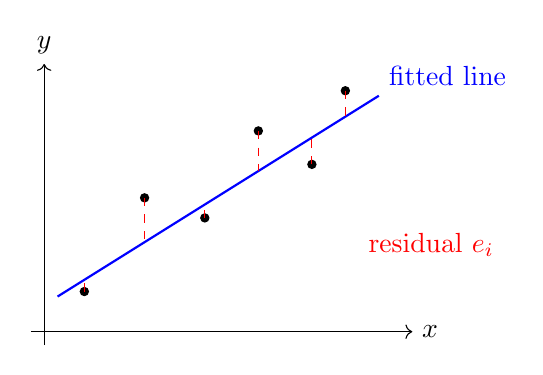
\begin{tikzpicture}[scale=0.85]
        \draw[->] (-0.2, 0) -- (5.5, 0) node[right] {$x$};
        \draw[->] (0, -0.2) -- (0, 4) node[above] {$y$};
        % fitted line: y = 0.4 + 0.625 x  (passes through (0.2, 0.525) and (5, 3.525))
        \draw[thick, blue] (0.2, 0.525) -- (5, 3.525) node[above right] {fitted line};
        % data points
        \foreach \x/\y in {0.6/0.6, 1.5/2.0, 2.4/1.7, 3.2/3.0, 4.0/2.5, 4.5/3.6} {
          \fill (\x, \y) circle (2pt);
        }
        % residuals as vertical dashed lines from data point to line
        \foreach \x/\y in {0.6/0.6, 1.5/2.0, 2.4/1.7, 3.2/3.0, 4.0/2.5, 4.5/3.6} {
          \pgfmathsetmacro\yhat{0.4 + 0.625*\x}
          \draw[red, dashed] (\x, \y) -- (\x, \yhat);
        }
        \node[red, anchor=west] at (4.7, 1.3) {residual $e_i$};
      \end{tikzpicture}
    \end{column}
  \end{columns}
\end{frame}

\subsection{The model}

\begin{frame}{The simple linear regression model}
  We model the response as a straight-line function of the predictor,
  plus random noise:
  \begin{block}{Formal model}
    \[
      \boxed{\,Y \;=\; \underbrace{\beta_0 + \beta_1 X}_{\text{signal (systematic)}}
             \;+\; \underbrace{\varepsilon}_{\text{noise (random)}}\,}
    \]
    with $E[\varepsilon] = 0$ and $\mathrm{Var}(\varepsilon) = \sigma^2$.
  \end{block}
  \begin{takeaway}[Signal plus noise]
    The line $\beta_0+\beta_1X$ is the part of $Y$ \emph{shared} by every
    observation at a given $X$; $\varepsilon$ is the part \emph{unique} to
    each one. Because the noise averages to zero, $Y \approx \beta_0 +
    \beta_1 X$ describes the \emph{typical} outcome at each $X$.
  \end{takeaway}
\end{frame}

\begin{frame}{Reading the model symbol-by-symbol}
  \begin{readme}
    \begin{tabular}{@{}cl@{}}
      \toprule
      \textbf{Symbol} & \textbf{Meaning} \\
      \midrule
      $Y$        & Response, the quantity we want to predict (e.g.\ sales). \\
      $X$        & Predictor / feature, the quantity we measure (e.g.\ TV spend). \\
      $\beta_0$  & Intercept: expected $Y$ when $X = 0$. \\
      $\beta_1$  & Slope: expected change in $Y$ for a 1-unit rise in $X$. \\
      $\varepsilon$ & Error: everything in $Y$ that $X$ does not explain. \\
      $\sigma^2$ & Variance of the error --- the noise floor. \\
      \bottomrule
    \end{tabular}
  \end{readme}
  $\beta_0, \beta_1, \sigma^2$ are unknown population parameters; we
  estimate them from the data and write the estimates with a hat:
  $\hat\beta_0$, $\hat\beta_1$, $\hat\sigma^2$.
\end{frame}

\begin{frame}{Predictions and residuals: definitions}
  Once we have estimates, two derived quantities matter on every slide
  for the rest of the chapter.
  \begin{block}{Fitted values}
    \[
      \hat y_i \;=\; \hat\beta_0 + \hat\beta_1 x_i.
    \]
    The line's prediction at $x_i$.
  \end{block}
  \begin{block}{Residuals}
    \[
      e_i \;=\; y_i - \hat y_i.
    \]
    What was left over --- the vertical mistake on observation $i$.
  \end{block}
  \begin{takeaway}
    Residuals are the workhorse of every diagnostic plot you will see.
    A good model has structureless residuals; structure in residuals
    is information the model is missing.
  \end{takeaway}
\end{frame}


\subsection{Estimating the line}

\begin{frame}{The principle: pick the line with smallest squared error}
  Among all possible $(\beta_0, \beta_1)$ we pick the one that
  minimises:
  \begin{block}{Residual sum of squares (RSS)}
    \[
      \mathrm{RSS}(\beta_0, \beta_1)
        \;=\; \sum_{i=1}^n \bigl(y_i - \beta_0 - \beta_1 x_i\bigr)^2.
    \]
  \end{block}
  \begin{readme}
    Each term in the sum is the vertical mistake for one observation,
    \emph{squared}. RSS adds them all up. We pick the line that makes
    this number smallest.
  \end{readme}
\end{frame}

\begin{frame}{The RSS surface: what least squares is minimising}
  \begin{center}
    
\includegraphics[width=0.96\textwidth,height=0.52\textheight,keepaspectratio]{ch03_x_rss_surface.png}
  \end{center}
  \begin{takeaway}[A single lowest point]
    $\mathrm{RSS}(\beta_0,\beta_1)$ is a convex \emph{bowl} over the plane
    of candidate coefficients. It has exactly one lowest point --- so
    there is a \emph{unique} best line, and the calculus on the next
    slides pins it down in closed form, with no trial-and-error search.
  \end{takeaway}
\end{frame}

\begin{frame}{Least-squares geometry: minimise the squared residuals}
  \begin{center}
    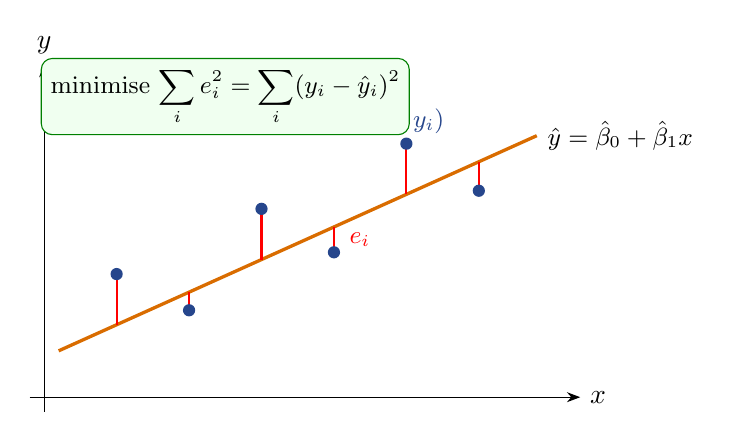
\begin{tikzpicture}[scale=0.92,>=Stealth]
      \draw[->] (-0.2,0) -- (7.4,0) node[right]{$x$};
      \draw[->] (0,-0.2) -- (0,4.6) node[above]{$y$};
      % fitted line: yhat = 0.55 + 0.45 x
      \draw[very thick,orange!85!black] (0.2,0.64) -- (6.8,3.61)
            node[right,black,font=\small]{$\hat y=\hat\beta_0+\hat\beta_1 x$};
      \foreach \x/\y in {1/1.7,2/1.2,3/2.6,4/2.0,5/3.5,6/2.85}{
        \pgfmathsetmacro\yh{0.55+0.45*\x}
        \draw[red,thick] (\x,\y) -- (\x,\yh);
        \fill[accent] (\x,\y) circle (2.4pt);
      }
      \pgfmathsetmacro\yhfour{0.55+0.45*4}
      \node[red,right,font=\small] at (4.08,{(2.0+\yhfour)/2}) {$e_i$};
      \node[accent,above,font=\small] at (5,3.5) {$(x_i,y_i)$};
      \node[draw=green!50!black,fill=green!6,rounded corners,align=center,
            font=\small] at (2.5,4.15)
            {minimise $\displaystyle\sum_{i} e_i^{2}=\sum_{i}(y_i-\hat y_i)^2$};
    \end{tikzpicture}
  \end{center}
  \begin{takeaway}
    Each red segment is a residual $e_i=y_i-\hat y_i$. OLS slides the
    line until the \emph{sum of squared} segment lengths is as small as
    possible --- larger misses are penalised more heavily.
  \end{takeaway}
\end{frame}

\begin{frame}{Why squared, and not absolute?}
  \begin{columns}[T]
    \begin{column}{0.48\textwidth}
      \textbf{Pros of squaring}
      \begin{itemize}
        \item Differentiable everywhere $\Rightarrow$ closed form.
        \item Larger mistakes punished more $\Rightarrow$ no huge
              residuals at the optimum.
        \item Aligns with the Gaussian-error likelihood (Gauss 1809).
      \end{itemize}
    \end{column}
    \begin{column}{0.48\textwidth}
      \textbf{Cons of squaring}
      \begin{itemize}
        \item Not robust to outliers --- one extreme $y_i$ can move
              the line a lot.
        \item Robust alternatives (median regression, Huber loss)
              exist and are useful when outliers dominate.
      \end{itemize}
    \end{column}
  \end{columns}
  \begin{takeaway}
    For a first course we always start with squared loss. Switching
    to robust losses is a one-line change in modern software.
  \end{takeaway}
\end{frame}

\begin{frame}{Deriving the slope: step 1 of 2}
  Set the partial derivative of RSS with respect to $\beta_1$ to zero:
  \[
    \frac{\partial \mathrm{RSS}}{\partial \beta_1}
      = -2 \sum_{i=1}^n x_i\,(y_i - \beta_0 - \beta_1 x_i) \;\stackrel{!}{=}\; 0.
  \]
  After simplifying (and using the equation for $\beta_0$ from the next
  step) we get the closed form:
  \[
    \boxed{\;
      \hat\beta_1
        = \frac{\sum_{i=1}^n (x_i - \bar x)(y_i - \bar y)}
               {\sum_{i=1}^n (x_i - \bar x)^2}
        = \frac{\widehat{\mathrm{cov}}(X, Y)}{\widehat{\mathrm{var}}(X)}.
    \;}
  \]
  \begin{readme}
    The slope is the sample covariance of $X$ and $Y$ divided by the
    sample variance of $X$. Strong covariation of $X$ and $Y$ pushes the slope up; more variation in
    $X$ (the denominator) pulls it back toward zero.
  \end{readme}
\end{frame}

\begin{frame}{Deriving the intercept: step 2 of 2}
  Set the partial derivative of RSS with respect to $\beta_0$ to zero:
  \[
    \frac{\partial \mathrm{RSS}}{\partial \beta_0}
      = -2 \sum_{i=1}^n (y_i - \beta_0 - \beta_1 x_i) \;\stackrel{!}{=}\; 0.
  \]
  Solve for $\beta_0$:
  \[
    \boxed{\;
      \hat\beta_0 = \bar y - \hat\beta_1 \bar x.
    \;}
  \]
  \begin{takeaway}[Two consequences for free]
    \begin{itemize}
      \item The fitted line always passes through $(\bar x, \bar y)$.
      \item The residuals sum to zero by construction; they are
            uncorrelated with $X$.
    \end{itemize}
  \end{takeaway}
\end{frame}

\begin{frame}{A concrete worked example}
  Suppose we have just five data points (small enough to do by hand):
  \[
    (x_1, y_1), \ldots, (x_5, y_5)
      = (1, 2),\;(2, 3),\;(3, 5),\;(4, 4),\;(5, 6).
  \]
  Compute means: $\bar x = 3$, $\bar y = 4$.
  \begin{numexample}
    \[
      \sum (x_i - \bar x)(y_i - \bar y) = 9, \qquad
      \sum (x_i - \bar x)^2 = 10.
    \]
    Hence:
    \[
      \hat\beta_1 = \tfrac{9}{10} = 0.9, \qquad
      \hat\beta_0 = 4 - 0.9 \cdot 3 = 1.3.
    \]
    The fitted line is $\hat y = 1.3 + 0.9 x$. Sanity check at
    $x = 3$: $\hat y = 4 = \bar y$ \checkmark.
  \end{numexample}
\end{frame}

\begin{frame}{Geometric picture: 3D residuals on real data}
  \begin{center}
    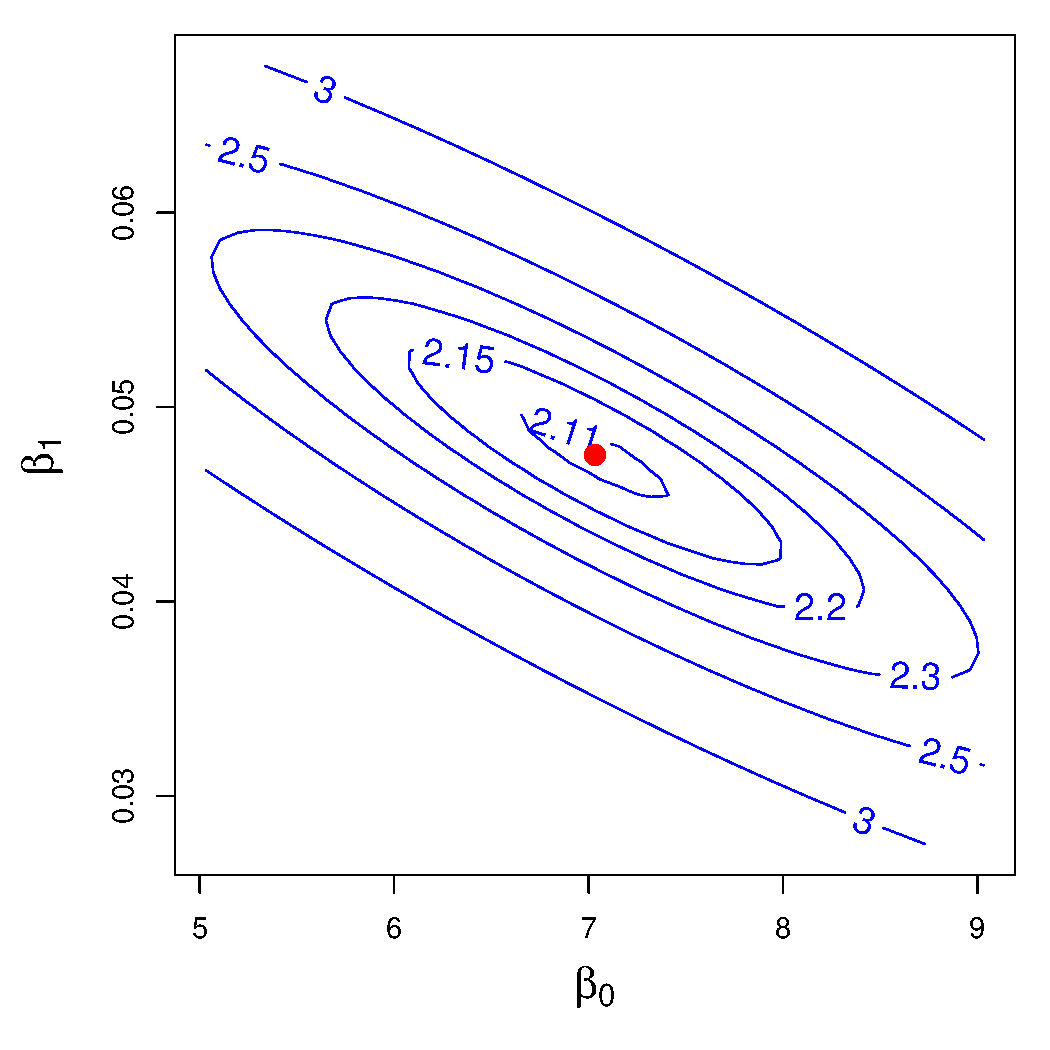
\includegraphics[width=0.85\textwidth,height=0.66\textheight,keepaspectratio]{3_2a.pdf}
  \end{center}
  Each red segment is a residual $e_i$. Least squares minimises the
  sum of the \emph{squared} red lengths --- not the sum of the lengths
  themselves.
  \islpsource{Figure 3.2}
\end{frame}

\begin{frame}{Recreating Figure 3.1 on the Advertising data}
  \begin{center}
    
\includegraphics[width=0.9\textwidth,height=0.62\textheight,keepaspectratio]{ch03_ols_residuals.png}
  \end{center}
  \begin{takeaway}
    The orange line is the OLS fit of \texttt{sales} on \texttt{TV}; each
    red segment is a residual $e_i$. Least squares picks the one line
    that makes the total \emph{squared} residual length smallest.
  \end{takeaway}
\end{frame}


% ============================================================
\begin{frame}{Exercise 3.1 --- Least squares by hand [Math]}
  \begin{exercise}
    You observe five data points:
    \[
      (x_i,y_i) = (1,3),\;(2,4),\;(3,2),\;(4,5),\;(5,6).
    \]
    \begin{enumerate}
      \item Compute the means $\bar x$ and $\bar y$.
      \item Compute $\sum (x_i-\bar x)(y_i-\bar y)$ and
            $\sum (x_i-\bar x)^2$, then the least-squares estimates
            $\hat\beta_1$ and $\hat\beta_0$.
      \item Write the fitted line and predict $y$ at $x=6$.
      \item Interpret the slope in words.
    \end{enumerate}
  \end{exercise}
\end{frame}

\begin{frame}{Solution --- Exercise 3.1 (1/2)}
  \begin{solutionbox}
    \emph{Method.} Every OLS quantity is built from deviations from the
    means, so we first compute $\bar x,\bar y$, then the co-movement
    $S_{xy}$ and the predictor spread $S_{xx}$.

    \textbf{(1) Means.}
    \[
      \bar x = \tfrac{1+2+3+4+5}{5}=3, \qquad
      \bar y = \tfrac{3+4+2+5+6}{5}=4.
    \]
    \textbf{(2) Cross-product and spread.} Tabulate deviations:
    \[
      \begin{array}{c|ccccc}
        x_i-\bar x & -2 & -1 & 0 & 1 & 2\\
        y_i-\bar y & -1 & 0 & -2 & 1 & 2
      \end{array}
    \]
    \[
      \sum (x_i-\bar x)(y_i-\bar y) = 2+0+0+1+4 = 7,\qquad
      \sum (x_i-\bar x)^2 = 4+1+0+1+4 = 10.
    \]
    Hence
    \[
      \hat\beta_1 = \frac{7}{10}=0.7,\qquad
      \hat\beta_0 = \bar y - \hat\beta_1\bar x = 4-0.7\cdot 3 = 1.9.
    \]
  \end{solutionbox}
\end{frame}

\begin{frame}{Solution --- Exercise 3.1 (2/2)}
  \begin{solutionbox}
    \textbf{(3) Fitted line and prediction.}
    \[
      \hat y = 1.9 + 0.7\,x, \qquad
      \hat y(6) = 1.9 + 0.7\cdot 6 = 6.1.
    \]
    Sanity check: at $x=\bar x=3$, $\hat y = 1.9+2.1 = 4 = \bar y$
    \checkmark\ (the line passes through $(\bar x,\bar y)$).

    \textbf{(4) Interpretation.} A one-unit increase in $x$ is
    associated with an average increase of $0.7$ units in $y$.
    The intercept $1.9$ is the predicted $y$ when $x=0$ (only
    meaningful if $x=0$ is within a sensible range).

    \medskip
    \textit{Common mistake:} treating $\hat y(6)=6.1$ as just as
    trustworthy as an in-range prediction. $x=6$ lies outside the
    observed range $[1,5]$, so this is (mild) extrapolation --- the
    further we move from the data, the less the fitted line can be
    trusted.
  \end{solutionbox}
\end{frame}

\subsection{Uncertainty}

\begin{frame}{Why estimates carry uncertainty}
  Our $\hat\beta_0$ and $\hat\beta_1$ were computed from a particular
  sample. A different sample from the same population would have
  produced slightly different estimates.
  \begin{takeaway}[Thought experiment]
    Imagine drawing 100 independent samples of 200 markets each and
    fitting OLS each time. We would get 100 different lines, each
    near but not on the true population line. The \emph{spread} of
    those 100 lines is the sampling variability we care about.
  \end{takeaway}
  Standard errors quantify this spread \emph{from a single sample}.
  Confidence intervals and hypothesis tests are built on top.
\end{frame}

\begin{frame}{Population vs.\ sample lines (illustration)}
  \begin{center}
    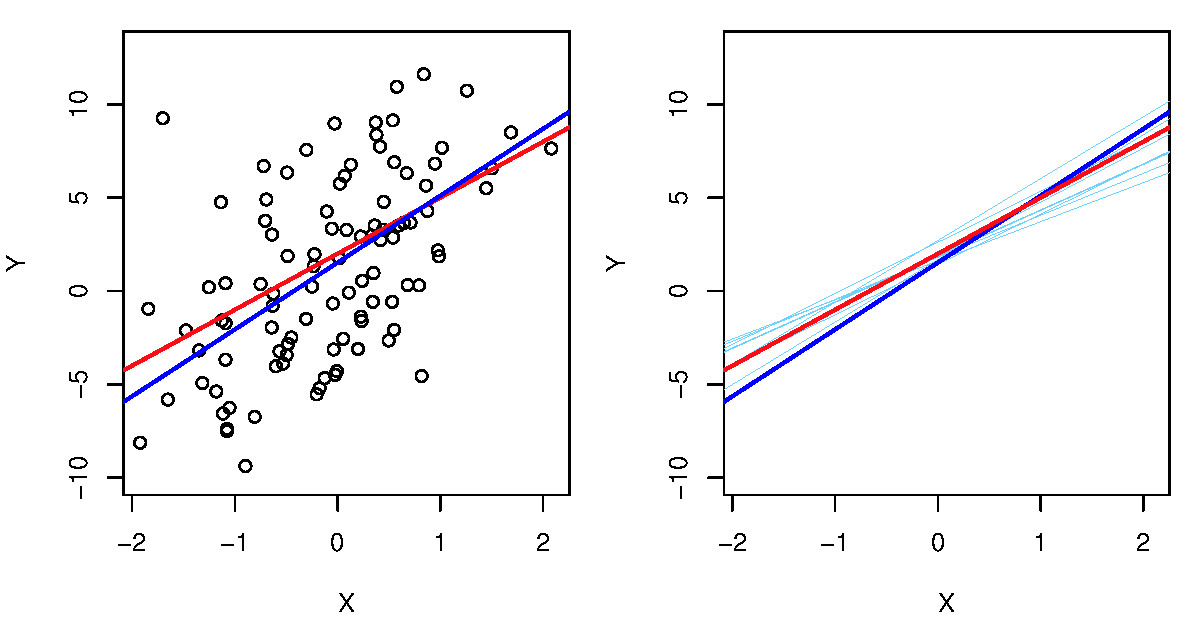
\includegraphics[width=0.72\textwidth,height=0.46\textheight,keepaspectratio]{3_3.pdf}
  \end{center}
  \begin{takeaway}
    The population line (red) is fixed but \emph{unobserved}; each sample
    line (blue) wobbles around it. A standard error measures that wobble
    from a \emph{single} sample --- we never see the red line itself.
  \end{takeaway}
  \islpsource{Figure 3.3}
\end{frame}

\begin{frame}{Standard errors of the OLS estimates}
  A \emph{standard error} measures how much an estimate would bounce
  around from one random sample to the next. Under the classical
  assumptions of independent errors with constant variance $\sigma^2$:
  \begin{block}{Formulas}
    \begin{align*}
      \mathrm{SE}(\hat\beta_0)^2
        &= \sigma^2\!\left[\,\tfrac{1}{n} +
            \tfrac{\bar x^2}{\sum (x_i - \bar x)^2}\,\right], \\[2pt]
      \mathrm{SE}(\hat\beta_1)^2
        &= \frac{\sigma^2}{\sum (x_i - \bar x)^2}.
    \end{align*}
  \end{block}
  In practice $\sigma^2$ is replaced by
  $\hat\sigma^2 = \mathrm{RSS}/(n-2)$, the squared
  \emph{residual standard error}.
\end{frame}

\begin{frame}{Reading the standard-error formulas}
  \begin{readme}
    \begin{itemize}
      \item The \emph{denominator} of $\mathrm{SE}(\hat\beta_1)^2$ is
            $\sum (x_i - \bar x)^2$. \emph{More spread-out predictors
            $\Rightarrow$ smaller SE for the slope.} (Long lever arm.)
      \item Both formulas have $\sigma^2$ in the numerator. \emph{Less
            noise $\Rightarrow$ smaller SEs.} Obvious in hindsight.
      \item $\mathrm{SE}(\hat\beta_0)^2$ shrinks like $1/n$ in $n$, so
            \emph{more data $\Rightarrow$ tighter intercept estimate}.
    \end{itemize}
  \end{readme}
  \begin{takeaway}[Practical implication]
    If you can choose where to measure, \emph{spread the $x_i$'s widely}.
    A study that measures $x \in \{2, 3, 4\}$ produces a much less
    precise slope than one that measures $x \in \{1, 5, 10\}$.
  \end{takeaway}
\end{frame}

\begin{frame}{Confidence interval: construction}
  Approximately,
  \[
    \boxed{\;\hat\beta_1 \;\pm\; 2\cdot \mathrm{SE}(\hat\beta_1)\;}
  \]
  is a $95\,\%$ confidence interval for $\beta_1$. (Strictly, use
  $t_{0.025,\,n-2}$ instead of $2$.)
  \begin{numexample}[Advertising example]
    For TV: $\hat\beta_1 = 0.0475$, $\mathrm{SE}(\hat\beta_1) = 0.0027$.\\
    $95\,\%$ CI: $[0.0475 - 2\cdot 0.0027,\; 0.0475 + 2\cdot 0.0027]
                 = [0.0421,\; 0.0529]$.\\
    \emph{Reading:} a \$1{,}000 increase in TV spend is associated with
    between $42$ and $53$ extra units of sales, with $95\,\%$
    confidence.
  \end{numexample}
\end{frame}

\begin{frame}{A picture of the 95\% confidence interval}
  \begin{center}
  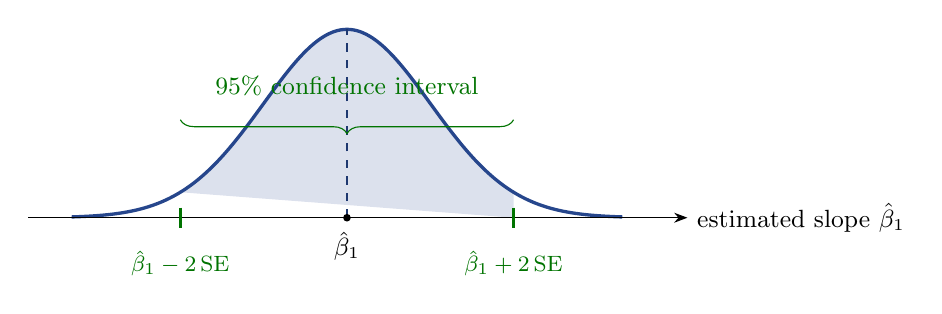
\begin{tikzpicture}[scale=0.92,>=Stealth]
    \def\amp{2.6}\def\ctr{5}\def\sd{1.15}
    \pgfmathsetmacro\muL{\ctr-2*\sd}
    \pgfmathsetmacro\muR{\ctr+2*\sd}
    % shaded 95% band under the sampling density
    \path[fill=accent!16] (\muL,0)
      plot[domain=\muL:\muR,samples=60,smooth]
        (\x,{\amp*exp(-(\x-\ctr)*(\x-\ctr)/(2*\sd*\sd))})
      -- (\muR,0) -- cycle;
    % sampling distribution of beta1-hat
    \draw[very thick,accent,domain=1.2:8.8,samples=100,smooth]
      plot (\x,{\amp*exp(-(\x-\ctr)*(\x-\ctr)/(2*\sd*\sd))});
    \draw[->] (0.6,0) -- (9.7,0) node[right,font=\small]{estimated slope $\hat\beta_1$};
    \draw[dashed,accent!80!black] (\ctr,0) -- (\ctr,\amp);
    \fill (\ctr,0) circle (1.5pt);
    \node[below,font=\small] at (\ctr,-0.06) {$\hat\beta_1$};
    \draw[very thick,green!45!black] (\muL,0.14) -- (\muL,-0.14);
    \draw[very thick,green!45!black] (\muR,0.14) -- (\muR,-0.14);
    \node[below,green!45!black,font=\footnotesize] at (\muL,-0.32) {$\hat\beta_1-2\,\mathrm{SE}$};
    \node[below,green!45!black,font=\footnotesize] at (\muR,-0.32) {$\hat\beta_1+2\,\mathrm{SE}$};
    \draw[decorate,decoration={brace,amplitude=5pt},green!45!black]
      (\muR,{\amp*0.52}) -- (\muL,{\amp*0.52})
      node[midway,above=5pt,green!45!black,font=\small]{95\% confidence interval};
  \end{tikzpicture}
  \end{center}
  \begin{takeaway}[Reading the picture]
    The bell is the sampling distribution of $\hat\beta_1$; the shaded
    band $\hat\beta_1\pm 2\,\mathrm{SE}$ is the 95\% confidence interval.
    The $t$-test asks the yes/no version of the same question ---
    \emph{does $0$ fall outside this band?} --- and if it does, the slope
    is significant at the $5\%$ level.
  \end{takeaway}
\end{frame}

\begin{frame}{Confidence interval: interpretation pitfalls}
  \begin{alertblock}{Common misreading}
    ``There is a $95\,\%$ probability that $\beta_1$ lies in $[a, b]$.''
    \\[2pt]
    This is \emph{wrong} under classical (frequentist) inference.
  \end{alertblock}
  \begin{readme}[Correct interpretation]
    The probability statement is about the random \emph{interval}, not
    the fixed parameter $\beta_1$:
    \begin{quote}
      \emph{If we repeated the experiment many times, $95\,\%$ of the
      constructed intervals would contain the true $\beta_1$.}
    \end{quote}
    For a Bayesian probability statement about $\beta_1$ given the
    data, you would need a prior and a posterior.
  \end{readme}
\end{frame}


% ============================================================
\begin{frame}{Exercise 3.2 --- Standard error, $t$ and CI [Math]}
  \begin{exercise}
    A simple linear regression is fit on $n=10$ observations. You are
    given $\hat\beta_1 = 2.5$, residual standard error
    $\mathrm{RSE}=4.0$, and $\sum(x_i-\bar x)^2 = 16$.
    \begin{enumerate}
      \item Compute the standard error
            $\mathrm{SE}(\hat\beta_1)=\mathrm{RSE}/\sqrt{\sum(x_i-\bar x)^2}$.
      \item Compute the $t$-statistic for $H_0:\beta_1=0$.
      \item Build a 95\% confidence interval for $\beta_1$
            (use $t_{0.025,\,8}=2.306$).
      \item Is the slope significant at the 5\% level? Justify.
    \end{enumerate}
  \end{exercise}
\end{frame}

\begin{frame}{Solution --- Exercise 3.2}
  \begin{solutionbox}
    \textbf{(1) Standard error.}
    \[
      \mathrm{SE}(\hat\beta_1)=\frac{\mathrm{RSE}}{\sqrt{\sum(x_i-\bar x)^2}}
        =\frac{4.0}{\sqrt{16}}=\frac{4.0}{4}=1.0.
    \]
    \textbf{(2) $t$-statistic.}
    \[
      t=\frac{\hat\beta_1-0}{\mathrm{SE}(\hat\beta_1)}
       =\frac{2.5}{1.0}=2.5,\qquad \text{df}=n-2=8.
    \]
    \textbf{(3) 95\% confidence interval.}
    \[
      \hat\beta_1 \pm t_{0.025,8}\cdot\mathrm{SE}(\hat\beta_1)
      = 2.5 \pm 2.306\cdot 1.0 = [\,0.194,\; 4.806\,].
    \]
    \textbf{(4) Significance.} $|t|=2.5 > 2.306$, equivalently the CI
    excludes $0$. We reject $H_0:\beta_1=0$ at the 5\% level; the
    two-sided $p$-value ($\approx 0.037$) is below $0.05$. There is
    evidence of a real linear association between $x$ and $y$.

    \medskip
    \textit{Note:} with only $n=10$ the critical value $2.306$ is well
    above the large-sample value $1.96$; small samples demand larger
    $t$'s to reach significance.
  \end{solutionbox}
\end{frame}

\subsection{Hypothesis tests}

\begin{frame}{The first question: is there \emph{any} relationship?}
  Before we do anything fancy, we test whether the predictor has any
  effect at all.
  \begin{block}{Hypotheses}
    \[
      H_0: \beta_1 = 0 \qquad \text{vs.} \qquad H_1: \beta_1 \ne 0.
    \]
  \end{block}
  In English: ``\emph{TV has no effect on sales}'' against
  ``\emph{TV has \emph{some} effect on sales}''.
  \begin{takeaway}[Why start here]
    If $\beta_1=0$ the line is flat and $X$ tells us nothing about $Y$.
    Rejecting $H_0$ is what \emph{licenses} interpreting the slope at all
    --- so this test comes \emph{before} we read off effect sizes or
    build confidence intervals.
  \end{takeaway}
\end{frame}

\begin{frame}{The $t$-statistic, step by step}
  \begin{block}{Test statistic}
    \[
      t \;=\; \frac{\hat\beta_1 - 0}{\mathrm{SE}(\hat\beta_1)}
            \;\sim\; t_{n-2} \text{ under } H_0.
    \]
  \end{block}
  \begin{readme}
    Numerator: \emph{how far} from zero is our estimate?
    Denominator: \emph{how surprising} would such a deviation be by
    sampling fluctuation alone?
    A large $|t|$ says: ``too far from zero to be a coincidence.''
  \end{readme}
  \begin{numexample}[Advertising TV regression]
    $t = 0.0475 / 0.0027 \approx 17.6$. The two-sided $p$-value is
    essentially zero --- we reject the null at any reasonable level.
  \end{numexample}
\end{frame}

\begin{frame}{Reading the regression output}
  \begin{center}
  \begin{tabular}{lrrrr}
    \toprule
    & Coef.\ & Std.\ Err.\ & $t$ & $p$ \\
    \midrule
    Intercept & $7.0325$ & $0.4578$ & $15.36$ & $<0.0001$ \\
    TV        & $0.0475$ & $0.0027$ & $17.67$ & $<0.0001$ \\
    \bottomrule
  \end{tabular}
  \end{center}
  \begin{readme}
    \begin{itemize}
      \item Each \$1{,}000 of TV advertising is associated with about
            $47.5$ extra units of sales on average.
      \item The slope is highly statistically significant
            ($t = 17.67$).
      \item The intercept (about $7{,}032$ units of sales when TV $= \$0$)
            is also significantly different from zero --- there is a
            non-zero baseline of sales.
    \end{itemize}
  \end{readme}
\end{frame}


\subsection{Goodness of fit}

\begin{frame}{Two summary measures of fit}
  After fitting any regression we want to know how well it fits.
  \begin{block}{Residual standard error (RSE)}
    \[
      \mathrm{RSE} \;=\; \sqrt{\frac{\mathrm{RSS}}{n - 2}}.
    \]
    The average size of a residual, in the units of $Y$. Smaller is
    better.
  \end{block}
  \begin{block}{Coefficient of determination $R^2$}
    \[
      R^2 \;=\; 1 - \frac{\mathrm{RSS}}{\mathrm{TSS}}, \quad
      \mathrm{TSS} = \sum (y_i - \bar y)^2.
    \]
    Proportion of variance in $Y$ that the model explains.
  \end{block}
\end{frame}

\begin{frame}{$R^2$: how to read it}
  \begin{readme}
    $R^2$ ranges between $0$ and $1$ in simple linear regression.
    \begin{itemize}
      \item $R^2 = 1$: model explains all variation in $Y$. The points
            sit exactly on the line.
      \item $R^2 = 0$: knowing $X$ tells us nothing about $Y$.
      \item In simple linear regression $R^2 = \mathrm{cor}(X, Y)^2$.
    \end{itemize}
  \end{readme}
  \begin{numexample}[Advertising TV regression]
    $\mathrm{RSE} = 3.26$, $R^2 = 0.61$. Translation: typical
    prediction is off by $3{,}260$ units of sales; the model explains
    $61\,\%$ of the variability in sales across markets.
  \end{numexample}
\end{frame}

\begin{frame}{Common misinterpretations of $R^2$}
  \begin{alertblock}{High $R^2$ does \emph{not} prove}
    \begin{itemize}
      \item the model is \emph{correct},
      \item the predictors \emph{cause} $Y$,
      \item the model will \emph{predict well} on new data.
    \end{itemize}
  \end{alertblock}
  \begin{alertblock}{Low $R^2$ does \emph{not} prove}
    \begin{itemize}
      \item the model is \emph{useless} --- in finance an $R^2$ of $0.05$
            can be very valuable,
      \item the predictors are \emph{irrelevant},
      \item there is \emph{no signal} to be found.
    \end{itemize}
  \end{alertblock}
\end{frame}


% ============================================================
\begin{frame}{Exercise 3.3 --- $R^2$, RSE and $\mathrm{cor}^2$ [Concept]}
  \begin{exercise}
    For the five points of Exercise~3.1 the fit gave
    $\mathrm{TSS}=\sum(y_i-\bar y)^2 = 10$ and
    $\mathrm{RSS}=\sum(y_i-\hat y_i)^2 = 5.1$ with $n=5$.
    \begin{enumerate}
      \item Compute $R^2$ and state in words what it means.
      \item Compute the residual standard error
            $\mathrm{RSE}=\sqrt{\mathrm{RSS}/(n-2)}$ and give its units
            interpretation.
      \item Recall $\mathrm{cor}(x,y)=0.7$. Verify the identity
            $R^2=\mathrm{cor}(x,y)^2$ that holds in simple linear
            regression, and explain why $R^2$ alone can be misleading.
    \end{enumerate}
  \end{exercise}
\end{frame}

\begin{frame}{Solution --- Exercise 3.3 (1/2)}
  \begin{solutionbox}
    \textbf{(1) Coefficient of determination.}
    \[
      R^2 = 1-\frac{\mathrm{RSS}}{\mathrm{TSS}} = 1-\frac{5.1}{10}=0.49.
    \]
    So $49\%$ of the variance of $y$ is explained by the linear fit on
    $x$; the remaining $51\%$ is unexplained (noise or missing
    structure).

    \textbf{(2) Residual standard error.}
    \[
      \mathrm{RSE}=\sqrt{\frac{\mathrm{RSS}}{n-2}}
        =\sqrt{\frac{5.1}{3}}=\sqrt{1.7}\approx 1.30.
    \]
    RSE is measured in the \emph{units of $y$}: a typical prediction
    misses the observed value by about $1.30$ units. Unlike $R^2$ it is
    not scale-free.
  \end{solutionbox}
\end{frame}

\begin{frame}{Solution --- Exercise 3.3 (2/2)}
  \begin{solutionbox}
    \textbf{(3) Identity.} Substituting the given correlation:
    \[
      \mathrm{cor}(x,y)^2 = 0.7^2 = 0.49 = R^2. \checkmark
    \]
    \emph{Why it holds:} with one predictor the fitted values are a
    linear function of $x$ ($\hat y=\hat\beta_0+\hat\beta_1 x$), so
    $\mathrm{cor}(y,\hat y)=|\mathrm{cor}(x,y)|$; and in any OLS fit
    with an intercept, $R^2=\mathrm{cor}(y,\hat y)^2$. With several
    predictors only the latter survives, so the identity is special to
    \emph{simple} regression.

    \emph{Why $R^2$ alone can mislead:} it can be high even when the
    linear form is wrong (curvature masked by a strong trend), and it
    never decreases when predictors are added --- so a large $R^2$ is
    not by itself evidence of a good or useful model. Check the
    residual plot and the RSE as well.

    \medskip
    \textit{Common mistake:} reading $R^2=0.49$ as ``49\% of points
    are predicted correctly''. It is the share of \emph{variance}
    explained --- a statement about spread, not about hit rates.
  \end{solutionbox}
\end{frame}

% ---------------- Extended Exercise 3.L1 [Math] ----------------
\begin{frame}{Extended Exercise 3.L1 --- Simple regression from A to Z [Math]}
  \begin{longexercise}
    A dealer records the resale value $y$ (in \$1000s) of a used car
    against its age $x$ (in years) for six cars:
    \[
      \begin{array}{c|cccccc}
        x_i\ (\text{age})   & 1 & 2 & 3 & 4 & 5 & 6\\ \hline
        y_i\ (\text{value}) & 19 & 18 & 17 & 15 & 12 & 9
      \end{array}
    \]
    Carry out a \emph{complete} simple linear regression by hand:
    \begin{enumerate}
      \item Estimate $\hat\beta_0,\hat\beta_1$ and write the fitted line.
      \item Compute the fitted values, residuals, RSS, RSE and $R^2$.
      \item Compute $\mathrm{SE}(\hat\beta_1)$, the $t$-statistic and the
            $95\%$ confidence interval for $\beta_1$.
      \item Predict the value of a $7$-year-old car with a $95\%$
            \emph{prediction} interval. Interpret every number.
    \end{enumerate}
    Useful: $t_{0.025,\,4}=2.776$.
  \end{longexercise}
\end{frame}

\begin{frame}{Solution --- Extended Exercise 3.L1 (1/3)}
  \begin{solutionbox}
    \textbf{Summaries.} $n=6$, $\bar x=3.5$, $\bar y=15$. With
    $x_i-\bar x=(-2.5,-1.5,-0.5,0.5,1.5,2.5)$ and
    $y_i-\bar y=(4,3,2,0,-3,-6)$,
    \[
      S_{xy}=\sum(x_i-\bar x)(y_i-\bar y)=-35,\quad
      S_{xx}=\sum(x_i-\bar x)^2=17.5,\quad
      S_{yy}=\sum(y_i-\bar y)^2=74.
    \]
    \textbf{(1) Slope, intercept, line.}
    \[
      \hat\beta_1=\frac{S_{xy}}{S_{xx}}=\frac{-35}{17.5}=-2,\qquad
      \hat\beta_0=\bar y-\hat\beta_1\bar x=15-(-2)(3.5)=22.
    \]
    \[
      \boxed{\ \hat y = 22 - 2\,x\ }\qquad
      \text{each extra year of age lowers value by }\$2000.
    \]
  \end{solutionbox}
\end{frame}

\begin{frame}{Solution --- Extended Exercise 3.L1 (2/3)}
  \begin{solutionbox}
    \textbf{(2) Fit quality.} Fitted $\hat y_i=(20,18,16,14,12,10)$;
    residuals $e_i=(-1,0,1,1,0,-1)$.
    \[
      \mathrm{RSS}=\sum e_i^2=4,\qquad
      \mathrm{RSE}=\sqrt{\tfrac{\mathrm{RSS}}{n-2}}=\sqrt{\tfrac{4}{4}}=1.0,\qquad
      R^2=1-\frac{\mathrm{RSS}}{S_{yy}}=1-\frac{4}{74}=0.946.
    \]
    Interpretation: a typical prediction misses the true value by about
    $\mathrm{RSE}=\$1000$; age alone explains $R^2=94.6\%$ of the
    variation in resale value.

    \textbf{(3) Inference on the slope.}
    \[
      \mathrm{SE}(\hat\beta_1)=\frac{\mathrm{RSE}}{\sqrt{S_{xx}}}
      =\frac{1}{\sqrt{17.5}}=0.239,\qquad
      t=\frac{\hat\beta_1}{\mathrm{SE}(\hat\beta_1)}=\frac{-2}{0.239}=-8.37.
    \]
    Since $|t|=8.37\gg 2.776$, we reject $H_0:\beta_1=0$: age is a highly
    significant predictor of value.
  \end{solutionbox}
\end{frame}

\begin{frame}{Solution --- Extended Exercise 3.L1 (3/3)}
  \begin{solutionbox}
    \textbf{95\% CI for $\beta_1$.}
    \[
      \hat\beta_1\pm t_{0.025,4}\,\mathrm{SE}(\hat\beta_1)
      =-2\pm 2.776(0.239)=[-2.66,\,-1.34].
    \]
    We are $95\%$ confident the annual drop is between \$1340 and \$2660;
    the interval excludes $0$, matching the $t$-test.

    \textbf{(4) Prediction at $x_0=7$.} $\hat y_0=22-2(7)=8$
    (\$8000). A \emph{prediction} interval for one new car adds the
    irreducible error (the ``$1+$''):
    \[
      \hat y_0\pm t\,\mathrm{RSE}\sqrt{1+\tfrac1n+\tfrac{(x_0-\bar x)^2}{S_{xx}}}
      =8\pm 2.776(1)\sqrt{1+\tfrac16+\tfrac{12.25}{17.5}}=8\pm 3.79,
    \]
    i.e.\ $[4.21,\,11.79]$ (\$4210--\$11{,}790). It is wide because $n$ is
    small, $x_0=7$ extrapolates beyond the data, and it targets a
    \emph{single} car rather than the average.
  \end{solutionbox}
\end{frame}

% ---------------- Extended Exercise 3.L2 [Math] ----------------
\begin{frame}{Extended Exercise 3.L2 --- Deriving least squares [Math]}
  \begin{longexercise}
    Do not merely \emph{use} the OLS formulas --- \emph{derive} them.
    \begin{enumerate}
      \item Write $\mathrm{RSS}(\beta_0,\beta_1)=\sum_{i=1}^{n}(y_i-\beta_0-\beta_1 x_i)^2$
            and set both partial derivatives to zero to obtain the
            \emph{normal equations}.
      \item Solve them for $\hat\beta_0$ and $\hat\beta_1$.
      \item Show the fitted line always passes through $(\bar x,\bar y)$.
      \item State precisely what it means that $\hat\beta_1$ is
            \emph{unbiased}.
      \item Plug in the summaries $n=20$, $\bar x=5$, $\bar y=15$,
            $S_{xx}=40$, $S_{xy}=100$ to get the estimates.
    \end{enumerate}
  \end{longexercise}
\end{frame}

\begin{frame}{Solution --- Extended Exercise 3.L2 (1/3)}
  \begin{solutionbox}
    \emph{Method.} $\mathrm{RSS}(\beta_0,\beta_1)$ is a smooth convex
    function of the two coefficients (a bowl), so its unique minimiser
    is the point where \emph{both} partial derivatives vanish --- two
    linear equations in two unknowns.

    \textbf{(1) Normal equations.} Differentiate the sum of squares and
    set each derivative to zero:
    \[
      \frac{\partial \mathrm{RSS}}{\partial \beta_0}
        =-2\sum (y_i-\beta_0-\beta_1 x_i)=0
        \;\Rightarrow\; \sum y_i=n\beta_0+\beta_1\sum x_i,
    \]
    \[
      \frac{\partial \mathrm{RSS}}{\partial \beta_1}
        =-2\sum x_i(y_i-\beta_0-\beta_1 x_i)=0
        \;\Rightarrow\; \sum x_i y_i=\beta_0\sum x_i+\beta_1\sum x_i^2.
    \]
    The factors $-2$ cancel. Read as statements about residuals: the
    first says the residuals sum to zero, the second says they are
    orthogonal to the predictor.
  \end{solutionbox}
\end{frame}

\begin{frame}{Solution --- Extended Exercise 3.L2 (2/3)}
  \begin{solutionbox}
    \textbf{(2) Solve the system.} Divide the first normal equation by
    $n$:
    \[
      \bar y=\beta_0+\beta_1\bar x
      \;\Rightarrow\; \hat\beta_0=\bar y-\hat\beta_1\bar x.
    \]
    Substitute this into the second equation (note
    $\sum x_i=n\bar x$) and collect the $\hat\beta_1$ terms:
    \[
      \sum x_i y_i=(\bar y-\hat\beta_1\bar x)\,n\bar x+\hat\beta_1\sum x_i^2
      \;\Rightarrow\;
      \sum x_i y_i-n\bar x\bar y
        =\hat\beta_1\Bigl(\sum x_i^2-n\bar x^2\Bigr).
    \]
    The centring identities
    $\sum x_i y_i-n\bar x\bar y=\sum(x_i-\bar x)(y_i-\bar y)=S_{xy}$ and
    $\sum x_i^2-n\bar x^2=\sum(x_i-\bar x)^2=S_{xx}$ then give
    \[
      \boxed{\ \hat\beta_1=\dfrac{\sum(x_i-\bar x)(y_i-\bar y)}{\sum(x_i-\bar x)^2}
      =\dfrac{S_{xy}}{S_{xx}}\ },\qquad
      \boxed{\ \hat\beta_0=\bar y-\hat\beta_1\bar x\ }.
    \]
    \textit{Common mistake:} trying to solve the second equation on its
    own --- the uncentred sums collapse to $S_{xy}/S_{xx}$ only
    \emph{after} substituting $\hat\beta_0=\bar y-\hat\beta_1\bar x$.
  \end{solutionbox}
\end{frame}

\begin{frame}{Solution --- Extended Exercise 3.L2 (3/3)}
  \begin{solutionbox}
    \textbf{(3) Passes through $(\bar x,\bar y)$.} At $x=\bar x$,
    \[
      \hat y=\hat\beta_0+\hat\beta_1\bar x
      =(\bar y-\hat\beta_1\bar x)+\hat\beta_1\bar x=\bar y.
    \]
    This is just the first normal equation restated --- the residuals
    always sum to zero.

    \textbf{(4) Unbiasedness.} Treating the $x_i$ as fixed and assuming
    $\mathbb{E}[\varepsilon_i]=0$, one shows $\mathbb{E}[\hat\beta_1]=\beta_1$
    and $\mathbb{E}[\hat\beta_0]=\beta_0$. Meaning: \emph{averaged over
    many repeated samples} the estimates are centred on the true values
    --- no systematic over- or under-estimation. (Any single estimate
    still has sampling error, quantified by its SE.)

    \textbf{(5) Plug in.}
    \[
      \hat\beta_1=\frac{S_{xy}}{S_{xx}}=\frac{100}{40}=2.5,\qquad
      \hat\beta_0=\bar y-\hat\beta_1\bar x=15-2.5(5)=2.5,
    \]
    so $\hat y=2.5+2.5\,x$.
  \end{solutionbox}
\end{frame}

% ============================================================
\section{Multiple Linear Regression}
% ============================================================
\subsection{From one predictor to many}

\begin{frame}{Why one predictor is rarely enough}
  Real applications rarely involve a single explanatory variable. The
  client cares about TV, radio, \emph{and} newspaper at once --- and
  they may interact.
  \begin{takeaway}
    Multiple regression lets us study the effect of one predictor
    \emph{while controlling for the others}. This ``ceteris paribus''
    interpretation is what makes regression so useful for inference.
  \end{takeaway}
  \begin{alertblock}{Why not just fit $p$ separate simple regressions?}
    Separate one-predictor fits cannot answer ``what is the effect of TV
    \emph{holding radio fixed}?'' If predictors move together, each
    isolated slope quietly absorbs the others' effects. One joint model
    disentangles them.
  \end{alertblock}
\end{frame}

\begin{frame}{The multiple linear regression model}
  \begin{block}{Formal model}
    \[
      \boxed{\;
        Y = \beta_0 + \beta_1 X_1 + \beta_2 X_2 + \cdots + \beta_p X_p
            + \varepsilon.
      \;}
    \]
  \end{block}
  Each $\beta_j$ is interpreted as:
  \begin{quote}
    \emph{The expected change in $Y$ for a one-unit increase in $X_j$,
    holding all other predictors fixed.}
  \end{quote}
  \begin{alertblock}{The clause that matters}
    The phrase ``holding others fixed'' is exactly what makes regression
    so useful for inference --- and so easy to misinterpret in the
    presence of confounders or collinearity.
  \end{alertblock}
\end{frame}

\begin{frame}{Matrix form: a compact view}
  Stack predictors into a design matrix $\mathbf{X}$ that includes a
  column of ones (for the intercept):
  \[
    \mathbf{y} \;=\; \mathbf{X}\,\boldsymbol\beta \;+\; \boldsymbol\varepsilon,
    \qquad
    \mathbf{X} \in \mathbb{R}^{n \times (p+1)}.
  \]
  Least squares gives the closed form
  \[
    \boxed{\;
      \hat{\boldsymbol\beta}
        \;=\; (\mathbf{X}^\top \mathbf{X})^{-1}\mathbf{X}^\top \mathbf{y}.
    \;}
  \]
  \begin{readme}
    \begin{itemize}
      \item $\mathbf{X}^\top\mathbf{X}$ must be invertible: requires
            $n > p + 1$ \emph{and} no perfect collinearity.
      \item The hat matrix $\mathbf{H} = \mathbf{X}(\mathbf{X}^\top\mathbf{X})^{-1}\mathbf{X}^\top$
            satisfies $\hat{\mathbf{y}} = \mathbf{H}\mathbf{y}$.
      \item Diagonal entries $h_{ii}$ are leverages --- we will use
            them in diagnostics.
    \end{itemize}
  \end{readme}
\end{frame}

% ============================================================
\begin{frame}[fragile]{Exercise 3.4 --- Multiple OLS on Advertising [Python]}
  \begin{exercise}
    Using \texttt{statsmodels}, fit
    $\texttt{sales} \sim \texttt{TV}+\texttt{radio}+\texttt{newspaper}$
    on the Advertising data.
    \begin{enumerate}
      \item Write the code to fit the model and print the summary.
      \item Given the estimated coefficients
            (intercept $2.94$, TV $0.0458$, radio $0.189$,
            newspaper $-0.001$), interpret the TV and radio slopes.
      \item Newspaper has a large $p$-value. What do you conclude, and
            how much extra sales does \$1000 of radio buy?
    \end{enumerate}
  \end{exercise}
\end{frame}

\begin{frame}[fragile]{Solution --- Exercise 3.4 (1/2)}
  \begin{solutionbox}
    \textbf{(1) Code.}
\begin{lstlisting}
import pandas as pd                  # data handling
import statsmodels.api as sm         # OLS with full inference output

ad = pd.read_csv("../../ALL CSV FILES - 2nd Edition/Advertising.csv",
                 index_col=0)        # load data; column 0 = row labels
X = sm.add_constant(ad[["TV", "radio", "newspaper"]])  # + intercept col
res = sm.OLS(ad["sales"], X).fit()   # fit sales on all three media
print(res.summary())                 # coef table: SE, t, p, R2, F
# TV ~ 0.0458, radio ~ 0.189, newspaper ~ -0.001 (p ~ 0.86)
# R-squared ~ 0.897
\end{lstlisting}
  \end{solutionbox}
\end{frame}

\begin{frame}{Solution --- Exercise 3.4 (2/2)}
  \begin{solutionbox}
    \textbf{(2) Interpretation (ceteris paribus).}
    Holding the other media fixed, spending an extra \$1000 on
    \emph{TV} is associated with about
    $0.0458\times 1000 = 45.8$ additional units sold; an extra \$1000 on
    \emph{radio} is associated with about
    $0.189\times 1000 = 189$ additional units. (Budgets are in
    thousands of dollars and sales in thousands of units.)

    \textbf{(3) Newspaper.} Its coefficient is essentially zero with a
    large $p$-value, so once TV and radio are in the model, newspaper
    adds no detectable predictive value. \$1000 of radio buys roughly
    $189$ extra units --- radio is far more effective per dollar than
    the tiny (non-significant) newspaper effect. The model explains
    about $90\%$ of the variance in sales ($R^2\approx 0.897$).

    \medskip
    \textit{Common mistake:} reading the near-zero newspaper slope as
    ``newspaper advertising can never work''. The model only says that
    \emph{given} TV and radio, newspaper adds no predictive value in
    these markets; its positive simple-regression slope arises because
    newspaper spend travels with radio spend (see Exercise~3.5).
  \end{solutionbox}
\end{frame}

\subsection{Confounding}

\begin{frame}{A cautionary tale: the Advertising slopes}
  Comparing single-predictor and multiple-predictor slopes side by side:
  \begin{center}
  \begin{tabular}{lrr}
    \toprule
    & Univariate slope & Multiple slope \\
    \midrule
    TV         & $\phantom{-}0.0475$ & $\phantom{-}0.0458$ \\
    Radio      & $\phantom{-}0.2025$ & $\phantom{-}0.1885$ \\
    Newspaper  & $\phantom{-}0.0547$ & $-0.0010$ \\
    \bottomrule
  \end{tabular}
  \end{center}
  \begin{alertblock}{What just happened?}
    Newspaper looks predictive on its own --- but its effect essentially
    \emph{disappears} once TV and radio are in the model. The univariate
    correlation came from newspaper spend co-moving with radio spend.
  \end{alertblock}
\end{frame}

\begin{frame}{Why a univariate $t$-test can mislead}
  \begin{takeaway}[Confounding in one sentence]
    Two predictors that move together can each look significant on
    their own, but only one of them actually drives the response.
  \end{takeaway}
  \begin{readme}[Practical rule]
    Always run \emph{multiple} regression when several predictors might
    be related to one another. Univariate $t$-tests are a useful
    diagnostic but not a substitute for joint analysis.
  \end{readme}
\end{frame}

% ============================================================
\begin{frame}{Exercise 3.5 --- Why newspaper ``works'' alone [Concept]}
  \begin{exercise}
    On the Advertising data, a \emph{simple} regression of sales on
    newspaper alone gives a positive, significant slope. But in the
    \emph{multiple} regression of Exercise~3.4 the newspaper
    coefficient is essentially zero and not significant. The correlation
    between newspaper and radio spending is about $0.35$.
    \begin{enumerate}
      \item Explain how newspaper can look helpful on its own yet be
            useless in the joint model.
      \item Which variable is the true driver, and what role is
            newspaper playing in the simple regression?
      \item State the general lesson for interpreting simple
            correlations.
    \end{enumerate}
  \end{exercise}
\end{frame}

\begin{frame}{Solution --- Exercise 3.5}
  \begin{solutionbox}
    \textbf{(1) Confounding.} Markets that spend more on radio also tend
    to spend somewhat more on newspaper ($\mathrm{cor}\approx 0.35$).
    Radio genuinely raises sales. In a simple regression, newspaper acts
    as a \emph{proxy} for the radio spending that travels with it, so it
    ``inherits'' a positive slope. Once radio is included in the multiple
    regression, radio absorbs that effect and newspaper's own
    coefficient collapses toward zero.

    \textbf{(2) True driver.} Radio (and TV) drive sales. In the simple
    regression newspaper is a surrogate / confounded stand-in for radio,
    not a cause of sales.

    \textbf{(3) General lesson.} A marginal (simple) association can be
    entirely due to correlation with an omitted variable. To assess the
    partial effect of a predictor --- its contribution holding others
    fixed --- you must include the other relevant predictors. Simple
    correlations invite confounding; ``correlation is not causation'' is
    the practical warning.
  \end{solutionbox}
\end{frame}

\subsection{The four important questions}

\begin{frame}{Four questions to ask of every multiple regression}
  After fitting any non-trivial linear model, ask:
  \begin{enumerate}
    \item Is at least one predictor useful? \hfill ($F$-test)
    \item Which subset of predictors is useful? \hfill ($t$-tests, Ch.~6)
    \item How well does the model fit the data? \hfill (RSE, $R^2$, plots)
    \item How accurate is a prediction at a new $x_0$? \hfill (CIs, PIs)
  \end{enumerate}
  Each question has a tailored statistical answer; we treat them in
  turn.
\end{frame}

\begin{frame}{Q1.\ Is \emph{any} predictor useful? --- the $F$-test}
  Test the joint null that no predictor matters at all:
  \[
    H_0: \beta_1 = \beta_2 = \cdots = \beta_p = 0.
  \]
  \begin{block}{$F$-statistic}
    \[
      F \;=\; \frac{(\mathrm{TSS} - \mathrm{RSS})/p}
                   {\mathrm{RSS}/(n - p - 1)}
            \;\sim\; F_{p,\,n-p-1} \text{ under } H_0.
    \]
  \end{block}
  \begin{readme}
    Numerator: \emph{average} reduction in RSS per added predictor.
    Denominator: \emph{average} residual variance per remaining degree
    of freedom. Large $F$ $\Rightarrow$ predictors are explaining more
    than chance.
  \end{readme}
\end{frame}

\begin{frame}{Why not just $p$ separate $t$-tests?}
  \begin{alertblock}{Multiple-testing inflation}
    With $p$ predictors and $\alpha = 0.05$ each, even under the
    \emph{global null} we expect $0.05 p$ rejections by chance alone.
    With $p = 20$ predictors that is one false positive per
    regression, on average.
  \end{alertblock}
  \begin{takeaway}
    The $F$-test handles this multiple-comparisons issue
    \emph{globally}. We will return to formal multiple-testing
    corrections in Chapter 13.
  \end{takeaway}
\end{frame}

\begin{frame}{Q2.\ Which predictors are useful?}
  This is the variable-selection question. Three approaches in
  increasing sophistication:
  \begin{block}{Approach 1: individual $t$-tests}
    Read off the regression table; useful when $p$ is small. Beware
    multiplicity.
  \end{block}
  \begin{block}{Approach 2: subset selection (Ch.~6)}
    Best subset, forward stepwise, backward stepwise. Use information
    criteria ($C_p$, AIC, BIC) or cross-validation to choose.
  \end{block}
  \begin{block}{Approach 3: regularisation (Ch.~6)}
    The lasso adds an $\ell_1$ penalty that shrinks irrelevant
    coefficients to exactly zero --- automatic variable selection.
  \end{block}
\end{frame}

\begin{frame}{Q3.\ How well does the model fit?}
  Three complementary tools:
  \begin{itemize}
    \item \textbf{Residual standard error (RSE):} typical residual
          magnitude in the units of $Y$ --- a concrete number.
    \item \textbf{$R^2$ (and adjusted $R^2$):} proportion of variance
          explained, useful for relative comparisons.
    \item \textbf{Residual plots:} structure in residuals signals model
          misspecification (next section).
  \end{itemize}
  \begin{alertblock}{Important nuance}
    Adding any predictor never \emph{decreases} $R^2$, even if the
    predictor is pure noise. \emph{Adjusted $R^2$} (Ch.~6) penalises
    this; cross-validation is more reliable still.
  \end{alertblock}
\end{frame}

\begin{frame}{Q4.\ How precise is a prediction?}
  At a new point $x_0$ we have two distinct uncertainty quantities:
  \begin{block}{Confidence interval for $E[Y \mid X = x_0]$}
    Quantifies the uncertainty in the \emph{regression line} at $x_0$.
    Narrows as $n \to \infty$.
  \end{block}
  \begin{block}{Prediction interval for an individual $Y_0$}
    Quantifies the uncertainty in the line \emph{plus} the inherent
    noise in $Y_0$. Includes $\sigma^2$ even at infinite $n$.
  \end{block}
  \begin{takeaway}[Key fact (often confused)]
    \emph{Prediction intervals are always wider than confidence
    intervals.} Use prediction intervals when communicating
    uncertainty about an individual outcome.
  \end{takeaway}
\end{frame}


% ============================================================
\begin{frame}{Exercise 3.6 --- The $F$-test vs.\ many $t$-tests [Math]}
  \begin{exercise}
    A multiple regression with $p=3$ predictors is fit on $n=100$
    observations, giving $\mathrm{TSS}=1000$ and $\mathrm{RSS}=100$.
    \begin{enumerate}
      \item Compute the overall $F$-statistic
            $F=\dfrac{(\mathrm{TSS}-\mathrm{RSS})/p}{\mathrm{RSS}/(n-p-1)}$.
      \item Compare with $F_{0.05,\,3,\,96}\approx 2.70$. What do you
            conclude?
      \item Suppose instead $p=100$ predictors were all truly useless.
            Roughly how many would appear ``significant'' at
            $\alpha=0.05$ using individual $t$-tests? Why does this
            motivate the $F$-test?
    \end{enumerate}
  \end{exercise}
\end{frame}

\begin{frame}{Solution --- Exercise 3.6}
  \begin{solutionbox}
    \textbf{(1) $F$-statistic.}
    \[
      F=\frac{(\mathrm{TSS}-\mathrm{RSS})/p}{\mathrm{RSS}/(n-p-1)}
       =\frac{(1000-100)/3}{100/(100-3-1)}
       =\frac{900/3}{100/96}
       =\frac{300}{1.0417}\approx 288.
    \]
    \textbf{(2) Conclusion.} $288 \gg 2.70$, so we overwhelmingly reject
    $H_0:\beta_1=\beta_2=\beta_3=0$. At least one predictor is related
    to the response.

    \textbf{(3) Multiple testing.} If all $100$ predictors are useless,
    each individual $t$-test still rejects with probability $\alpha=0.05$
    by chance, so we expect about $100\times 0.05 = 5$ ``significant''
    predictors purely from noise. Scanning many $t$-tests therefore
    almost guarantees false positives. The $F$-test gives a single
    overall test whose Type~I error stays at $\alpha$ regardless of $p$,
    which is why we consult it \emph{first} before looking at individual
    coefficients.
  \end{solutionbox}
\end{frame}

% ---------------- Extended Exercise 3.L3 [Python] ----------------
\begin{frame}[fragile]{Extended Exercise 3.L3 --- Multiple regression on Advertising [Python]}
  \begin{longexercise}
    Using \texttt{statsmodels} and \texttt{Advertising.csv}, fit the
    multiple regression
    $\texttt{sales}\sim\texttt{TV}+\texttt{radio}+\texttt{newspaper}$.
    \begin{enumerate}
      \item Fit the model and read the summary: interpret each slope, the
            overall $F$-test, and $R^2$ vs adjusted $R^2$.
      \item In a \emph{simple} regression $\texttt{sales}\sim\texttt{newspaper}$
            the newspaper slope is significant, yet here it is not.
            Explain the apparent contradiction (confounding).
      \item Drop newspaper and refit. Compare coefficients, $R^2$ and RSE.
            Which model do you keep, and why?
    \end{enumerate}
  \end{longexercise}
\end{frame}

\begin{frame}[fragile]{Solution --- Extended Exercise 3.L3 (1/3)}
  \begin{solutionbox}
    \textbf{(1) Fit and summary.}
\begin{lstlisting}
import pandas as pd, numpy as np, statsmodels.api as sm  # libraries
ad = pd.read_csv("../../ALL CSV FILES - 2nd Edition/Advertising.csv",
                 index_col=0)          # load data; col 0 = row labels
X   = sm.add_constant(ad[["TV", "radio", "newspaper"]])  # design + const
res = sm.OLS(ad["sales"], X).fit()     # least-squares fit
print(res.summary())                   # full inference table
# const 2.939 | TV 0.0458 (p<.001) | radio 0.189 (p<.001)
# newspaper -0.0010 (p=0.86, 95% CI [-0.013, 0.010])
# R2 = 0.897 | adj-R2 = 0.896 | F = 570.3 (p = 1.6e-96) | RSE = 1.686
\end{lstlisting}
  \end{solutionbox}
\end{frame}

\begin{frame}{Solution --- Extended Exercise 3.L3 (2/3)}
  \begin{solutionbox}
    \textbf{Reading it.} Holding the others fixed, \$1000 more on
    \emph{TV} adds $\approx 45.8$ units of sales and \$1000 more on
    \emph{radio} adds $\approx 188$ units; \emph{newspaper} is $\approx 0$
    ($p=0.86$; its CI straddles $0$). The $F$-statistic $570$ (tiny $p$)
    tests $H_0:\beta_{\text{TV}}=\beta_{\text{radio}}=\beta_{\text{news}}=0$
    and is decisively rejected --- at least one medium matters. Here
    $R^2=0.897$ and adjusted $R^2=0.896$ are almost equal because there
    are only three predictors.

    \textbf{(2) Why newspaper ``flips''.} Alone,
    $\texttt{sales}\sim\texttt{newspaper}$ has slope $0.055$ ($p=0.001$).
    But $\mathrm{cor}(\texttt{radio},\texttt{newspaper})=0.35$: markets
    with big radio budgets also buy more newspaper. Alone, newspaper acts
    as a \emph{proxy} for radio and borrows its effect; once radio is in
    the model, newspaper adds nothing. This is textbook \emph{confounding}.
  \end{solutionbox}
\end{frame}

\begin{frame}[fragile]{Solution --- Extended Exercise 3.L3 (3/3)}
  \begin{solutionbox}
    \textbf{(3) Drop newspaper and refit.}
\begin{lstlisting}
X2   = sm.add_constant(ad[["TV", "radio"]])  # drop newspaper column
res2 = sm.OLS(ad["sales"], X2).fit()         # refit the smaller model
# const 2.921 | TV 0.0458 | radio 0.188
# R2 = 0.897 (unchanged) | adj-R2 0.896 -> 0.896 | RSE 1.686 -> 1.681
\end{lstlisting}
    The TV and radio slopes barely move, $R^2$ is essentially unchanged,
    and RSE improves slightly. \textbf{Keep the two-predictor model}: it
    is simpler, loses no explanatory power, and both adjusted $R^2$ and
    RSE (which penalise useless predictors) favour it. Parsimony wins,
    and it agrees with the confounding diagnosis in part (2).
  \end{solutionbox}
\end{frame}

% ============================================================
\section{Extensions}
% ============================================================
\subsection{Qualitative predictors}

\begin{frame}{What if a predictor is categorical?}
  Many real predictors are categorical: gender, region, brand, day of
  the week. We cannot use them directly --- regression needs numbers.
  \begin{takeaway}[Solution: dummy coding]
    Replace a categorical predictor with one or more $0/1$ indicator
    variables. The math then works exactly as before.
  \end{takeaway}
  \begin{numexample}[Coding ``owns a home?'']
    \texttt{Own} $\in\{$Yes, No$\}$ becomes one column: $x=1$ for owners,
    $x=0$ for non-owners. Its coefficient is then the average
    $Y$-difference between owners and non-owners.
  \end{numexample}
\end{frame}

\begin{frame}{Two levels: a single 0/1 dummy}
  For a binary predictor with levels A and B:
  \[
    x_i = \begin{cases}
            1 & \text{if observation $i$ is in level A,} \\
            0 & \text{if in level B (the baseline).}
          \end{cases}
  \]
  \begin{readme}
    The coefficient $\beta_j$ is interpreted as the average difference
    in $Y$ between level A and the baseline B, holding all other
    predictors fixed. Either level can serve as baseline; only the
    sign of $\hat\beta_j$ flips.
  \end{readme}
\end{frame}

\begin{frame}{$K$ levels: use $K-1$ dummies}
  Use $K - 1$ dummy variables and let one level serve as the baseline.
  \begin{alertblock}{Why not $K$ dummies?}
    With $K$ dummies, the dummies sum to a column of ones --- collinear
    with the intercept. The design matrix would not be full rank and
    OLS would have no unique solution.
  \end{alertblock}
  \begin{numexample}[Three-region predictor]
    Suppose region $\in$ \{North, South, East\}. Set North as baseline.
    Use two dummies: $x_S = 1$ if South, $x_E = 1$ if East. The
    coefficients $\beta_S, \beta_E$ are the average $Y$-differences
    relative to North, holding others fixed.
  \end{numexample}
\end{frame}

% ============================================================
\begin{frame}{Exercise 3.7 --- Dummy coding factors [Math]}
  \begin{exercise}
    \begin{enumerate}
      \item \textbf{Two levels.} Regressing credit-card balance on a
            student indicator gives
            $\widehat{\texttt{balance}} = 480.4 + 396.5\cdot
            \texttt{student}$, where $\texttt{student}=1$ for students,
            $0$ otherwise. Give the predicted average balance for
            students and for non-students, and interpret $396.5$.
      \item \textbf{Three levels.} For region with East as the baseline
            and dummies for South and West, the fit is
            \[
              \widehat{\texttt{balance}} = 531 - 12.5\cdot\texttt{South}
                - 18.7\cdot\texttt{West}.
            \]
            Give the predicted mean balance in each region.
      \item Why do we use only $k-1$ dummies for a $k$-level factor?
    \end{enumerate}
  \end{exercise}
\end{frame}

\begin{frame}{Solution --- Exercise 3.7}
  \begin{solutionbox}
    \textbf{(1) Two levels.}
    \[
      \text{non-student }(\texttt{student}=0):\ \hat y = 480.4,\qquad
      \text{student }(\texttt{student}=1):\ \hat y = 480.4+396.5 = 876.9.
    \]
    The coefficient $396.5$ is the \emph{difference} in average balance:
    students carry, on average, \$396.5 more balance than non-students.
    The intercept $480.4$ is the baseline (non-student) mean.

    \textbf{(2) Three levels.} The intercept $531$ is the baseline
    (East) mean; each dummy coefficient is a difference from East.
    \[
      \text{East}=531,\qquad
      \text{South}=531-12.5=518.5,\qquad
      \text{West}=531-18.7=512.3.
    \]

    \textbf{(3) Why $k-1$ dummies.} A separate dummy for every level
    plus an intercept would be perfectly collinear (the dummies sum to
    the all-ones intercept column), so the design matrix is not full
    rank and the coefficients are not identified --- the ``dummy
    variable trap''. Dropping one level makes it the baseline that the
    intercept represents; the remaining $k-1$ coefficients are
    contrasts against that baseline. Overall differences among levels
    are still tested jointly with an $F$-test.
  \end{solutionbox}
\end{frame}

\subsection{Interactions}

\begin{frame}{Why a plain linear model can miss the truth}
  Plain linear regression assumes the effect of $X_1$ is the \emph{same}
  at every value of $X_2$. Often this is wrong.
  \begin{numexample}[A simple synergy]
    Spending \$50k on TV \emph{and} \$30k on radio yields more sales
    than spending \$50k on either alone. The two channels reinforce
    each other --- they \emph{interact}.
  \end{numexample}
  \begin{takeaway}
    The fix is to add a multiplicative term $X_1 X_2$ to the model.
  \end{takeaway}
\end{frame}

\begin{frame}{The interaction model}
  \begin{block}{Two predictors with an interaction}
    \[
      Y = \beta_0 + \beta_1 X_1 + \beta_2 X_2 + \beta_3\,X_1 X_2 + \varepsilon.
    \]
  \end{block}
  \begin{readme}
    Differentiate with respect to $X_1$:
    \[
      \frac{\partial Y}{\partial X_1} = \beta_1 + \beta_3 X_2.
    \]
    The slope in $X_1$ now depends on $X_2$ --- exactly the synergy we
    wanted to model.
  \end{readme}
\end{frame}

\begin{frame}{Interaction, drawn: one slope bends with the other predictor}
  \begin{columns}[T]
    \begin{column}{0.54\textwidth}
      \begin{center}
      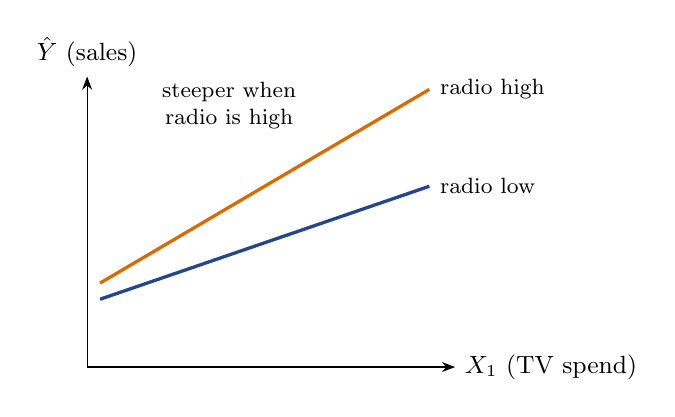
\begin{tikzpicture}[scale=0.82,>=Stealth]
        \draw[->] (0,0) -- (5.7,0) node[right,font=\small]{$X_1$ (TV spend)};
        \draw[->] (0,0) -- (0,4.5) node[above,font=\small]{$\hat Y$ (sales)};
        \draw[very thick,accent] (0.2,1.05) -- (5.3,2.80)
              node[right,font=\footnotesize,black]{radio low};
        \draw[very thick,orange!85!black] (0.2,1.30) -- (5.3,4.30)
              node[right,font=\footnotesize,black]{radio high};
        \node[align=center,font=\footnotesize] at (2.2,4.05)
              {steeper when\\radio is high};
      \end{tikzpicture}
      \end{center}
    \end{column}
    \begin{column}{0.44\textwidth}
      \begin{readme}
        The interaction makes the slope of $\hat Y$ in $X_1$ equal to
        $\hat\beta_1+\hat\beta_3 X_2$: different values of $X_2$ give lines
        with \emph{different slopes}, so they fan out instead of staying
        parallel.
      \end{readme}
      \begin{takeaway}
        Parallel lines $=$ no interaction. A fan $=$ synergy: the
        predictors amplify each other.
      \end{takeaway}
    \end{column}
  \end{columns}
\end{frame}

\begin{frame}{The hierarchy principle}
  \begin{alertblock}{Rule}
    If an interaction $X_1 X_2$ is in the model, keep the main effects
    $X_1$ and $X_2$ as well, even if their individual $t$-statistics
    are small.
  \end{alertblock}
  \begin{readme}[Why]
    Without main effects, the interaction is parameterising deviations
    from a model in which neither $X_1$ nor $X_2$ enters --- a strong
    and usually unintended assumption.
  \end{readme}
\end{frame}

\begin{frame}{Interaction plot for Advertising}
  \begin{center}
    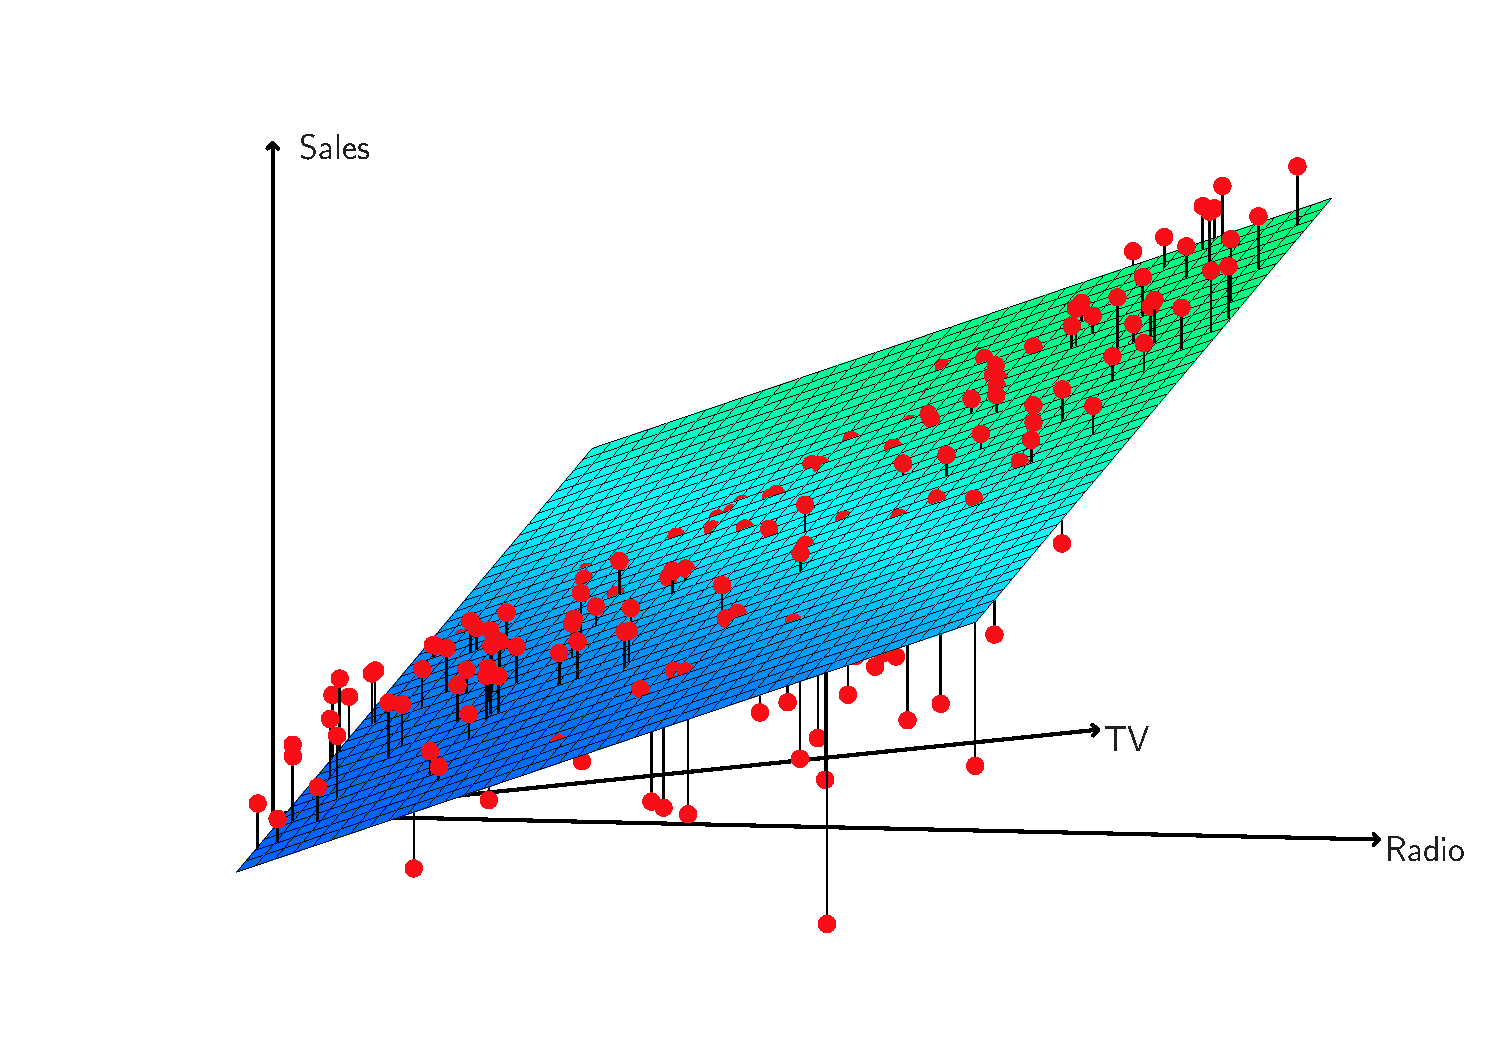
\includegraphics[width=0.72\textwidth,height=0.46\textheight,keepaspectratio]{3_5.pdf}
  \end{center}
  \begin{takeaway}[What the figure shows]
    A \texttt{TV}$\times$\texttt{radio} term lets the sales surface
    \emph{bend}: a dollar of TV returns more when radio is also high.
    Adding it lifts $R^2$ from about $0.90$ to $0.97$ on these data.
  \end{takeaway}
  \islpsource{Figure 3.5}
\end{frame}

% ============================================================
\begin{frame}{Exercise 3.8 --- Interactions and hierarchy [Concept]}
  \begin{exercise}
    On the Advertising data a model with an interaction gives
    \[
      \widehat{\texttt{sales}} = 6.75 + 0.019\,\texttt{TV}
        + 0.029\,\texttt{radio} + 0.0011\,(\texttt{TV}\times\texttt{radio}).
    \]
    \begin{enumerate}
      \item Interpret the interaction coefficient $0.0011$ in words.
      \item Compute the effective slope of TV when radio $=0$ and when
            radio $=50$.
      \item State the \emph{hierarchy principle}. If the TV main effect
            were not significant but $\texttt{TV}\times\texttt{radio}$
            were, should you drop TV?
    \end{enumerate}
  \end{exercise}
\end{frame}

\begin{frame}{Solution --- Exercise 3.8}
  \begin{solutionbox}
    \textbf{(1) Interaction meaning.} The effect of TV on sales is not
    constant --- it \emph{grows} with the radio budget (and vice versa).
    Concretely, each extra unit of radio raises the per-unit
    effectiveness of TV by $0.0011$. This is a \emph{synergy}: the two
    media reinforce each other.

    \textbf{(2) Effective TV slope.}
    \[
      \frac{\partial\,\widehat{\texttt{sales}}}{\partial\,\texttt{TV}}
        = 0.019 + 0.0011\cdot\texttt{radio}.
    \]
    \[
      \texttt{radio}=0:\ 0.019, \qquad
      \texttt{radio}=50:\ 0.019 + 0.0011\cdot 50 = 0.019+0.055 = 0.074.
    \]
    With a \$50k radio budget, TV is nearly four times as effective per
    dollar as with no radio.

    \textbf{(3) Hierarchy principle.} If an interaction term is included
    in a model, the corresponding main effects should be kept too, even
    if their individual $p$-values are large. So \emph{no} --- do not
    drop TV: the interaction $\texttt{TV}\times\texttt{radio}$ is not
    interpretable without the TV main effect, and removing it makes the
    remaining coefficients hard to read and can bias the fit.
  \end{solutionbox}
\end{frame}

\begin{frame}{Seeing the interaction: the TV slope depends on radio}
  \begin{center}
\includegraphics[width=0.88\textwidth,height=0.5\textheight,keepaspectratio]{ch03_x_tv_radio_interaction.png}\end{center}
  \begin{takeaway}On Advertising, an extra \$1k of TV is worth $0.030$ thousand units of sales when radio is at its 25th percentile but $0.059$ --- almost double --- at the 75th ($p_{\text{interaction}} \approx 10^{-51}$). Non-parallel fitted lines are the signature of synergy.\end{takeaway}
\end{frame}

\subsection{Polynomial extension}

\begin{frame}{Polynomial regression \emph{is} linear regression}
  Adding $X^2$, $X^3$, \ldots terms keeps the model \emph{linear in
  the coefficients}, even though the relationship $X \to Y$ is curved.
  \begin{block}{Quadratic in $X$, linear in $\beta$}
    \[
      Y = \beta_0 + \beta_1 X + \beta_2 X^2 + \varepsilon.
    \]
    All OLS machinery applies; we simply augment the design matrix.
  \end{block}
  \begin{takeaway}
    Polynomial regression is the cheapest way to capture mild
    curvature. It has known weaknesses (boundary oscillation), but
    splines (Ch.~7) are the better long-term answer.
  \end{takeaway}
\end{frame}

\begin{frame}{Auto: linear vs.\ quadratic fit}
  \begin{center}
    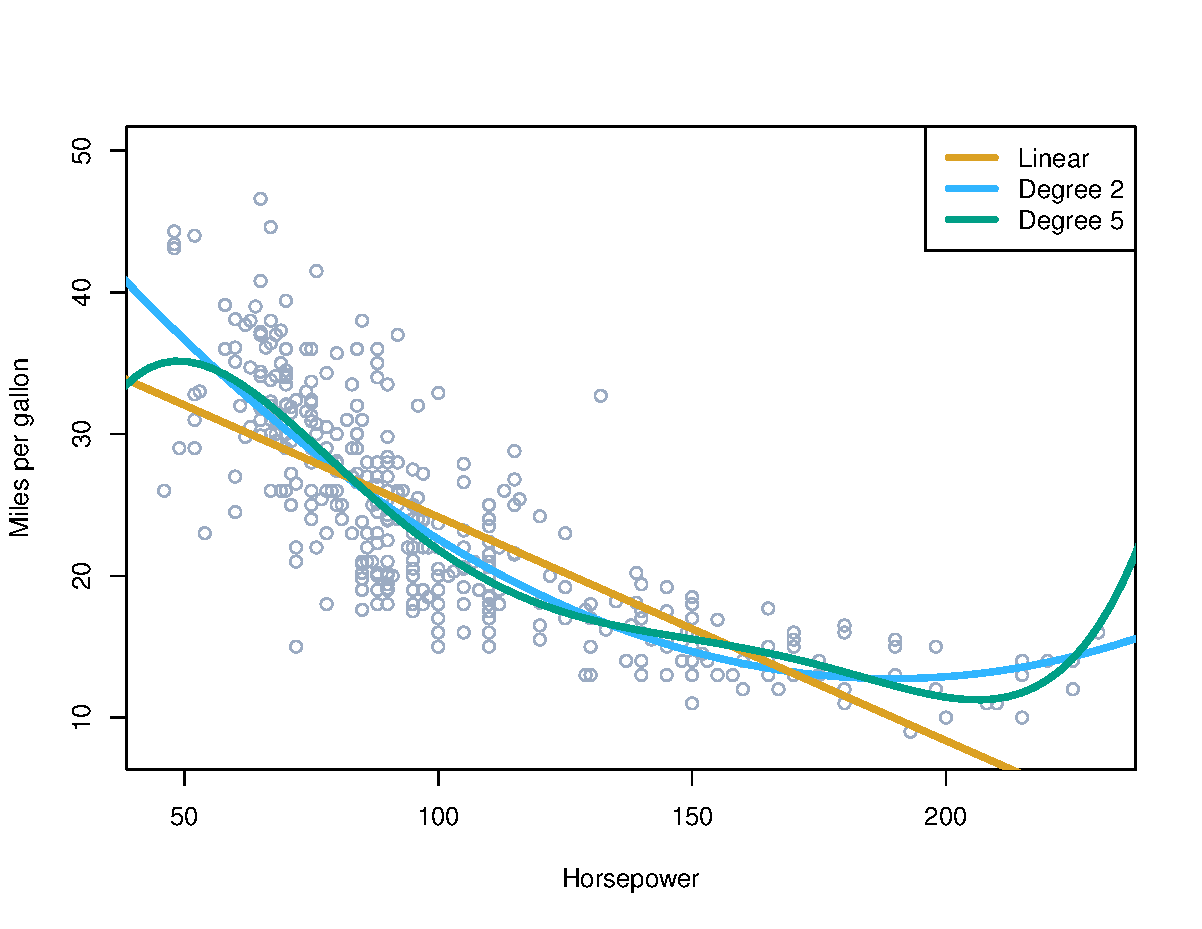
\includegraphics[width=0.72\textwidth,height=0.45\textheight,keepaspectratio]{3_8.pdf}
  \end{center}
  \begin{takeaway}
    Linear (orange) underfits --- a straight line cannot bend. The
    quadratic (blue) captures the curvature with one extra term. Past
    degree~4, flexibility adds variance and edge oscillation for little gain.
  \end{takeaway}
  \islpsource{Figure 3.8}
\end{frame}


\begin{frame}{Conceptual summary so far}
  \begin{takeaway}[Where we are in the chapter]
    We have built the linear model, learnt to estimate it, run inference,
    handled qualitative predictors and interactions, and explored
    polynomial extensions.
  \end{takeaway}
  \begin{readme}[The next step]
    A model is only as good as its diagnostics. We now learn to spot the
    four classical regression problems and what to do about them:
    nonlinearity, heteroscedasticity, outliers / leverage, collinearity.
  \end{readme}
\end{frame}

% ============================================================
\begin{frame}[fragile]{Exercise 3.9 --- Polynomial fit on Auto [Python]}
  \begin{exercise}
    Using the Auto data, model $\texttt{mpg}$ against
    $\texttt{horsepower}$.
    \begin{enumerate}
      \item Fit a linear model and a quadratic (degree-2) model with
            \texttt{statsmodels}.
      \item The linear fit gives $R^2\approx 0.606$; the quadratic gives
            $R^2\approx 0.688$ with a highly significant
            $\texttt{horsepower}^2$ term. What does this tell you about
            the relationship?
      \item Why is the quadratic model still called a \emph{linear}
            model?
    \end{enumerate}
  \end{exercise}
\end{frame}

\begin{frame}[fragile]{Solution --- Exercise 3.9 (1/2)}
  \begin{solutionbox}
    \textbf{(1) Code.}
    \vspace{-2mm}
\begin{lstlisting}
import pandas as pd, numpy as np
import statsmodels.api as sm

auto = pd.read_csv("../../ALL CSV FILES - 2nd Edition/Auto.csv",
                   na_values="?").dropna()  # "?" -> NaN, then drop
hp = auto["horsepower"].astype(float)       # ensure numeric predictor

# Linear model
X1 = sm.add_constant(hp)                    # intercept + hp
m1 = sm.OLS(auto["mpg"], X1).fit()          # fit mpg ~ hp

# Quadratic model
X2 = sm.add_constant(np.column_stack([hp, hp**2]))  # cols: hp, hp^2
m2 = sm.OLS(auto["mpg"], X2).fit()          # fit mpg ~ hp + hp^2

print(m1.rsquared, m2.rsquared)   # ~ 0.606 , ~ 0.688
\end{lstlisting}
  \end{solutionbox}
\end{frame}

\begin{frame}{Solution --- Exercise 3.9 (2/2)}
  \begin{solutionbox}
    \textbf{(2) Interpretation.} The jump from $R^2\approx 0.606$ to
    $0.688$ and the significant squared term show the relationship is
    \emph{curved}, not straight: mpg falls steeply as horsepower rises
    from low values, then flattens. A straight line systematically
    under- and over-predicts (a U-shaped residual pattern), which the
    quadratic term corrects.

    \textbf{(3) Still ``linear''.} The model is linear in the
    \emph{parameters}: $\texttt{mpg}=\beta_0+\beta_1\texttt{hp}
    +\beta_2\texttt{hp}^2+\varepsilon$ is linear in
    $\beta_0,\beta_1,\beta_2$ even though it is nonlinear in the
    predictor. We simply treat $\texttt{hp}^2$ as an additional
    predictor, so ordinary least squares still applies.

    \medskip
    \textit{Common mistake:} justifying the quadratic by the $R^2$
    increase alone --- $R^2$ \emph{never} decreases when a term is
    added. The real evidence is the highly significant $t$-statistic
    on $\texttt{hp}^2$ (here $t\approx 10$) together with the
    disappearance of the U-shape from the residual plot.
  \end{solutionbox}
\end{frame}

% ---------------- Extended Exercise 3.L4 [Integrative] ----------------
\begin{frame}{Extended Exercise 3.L4 --- Dummies and interactions [Integrative]}
  \begin{longexercise}
    A store models monthly \emph{spend} $y$ (in \$100s) from a customer's
    \emph{income} $x$ (in \$1000s) and \emph{region}, a 3-level factor
    (East, South, West). With East as baseline and dummies $D_S,D_W$, the
    model \emph{with interaction} is
    \[
      y=\beta_0+\beta_1 x+\beta_2 D_S+\beta_3 D_W
        +\beta_4 (x\!\cdot\!D_S)+\beta_5 (x\!\cdot\!D_W)+\varepsilon,
    \]
    and the fit gives $(\hat\beta_0,\dots,\hat\beta_5)=(30,\,6,\,-10,\,20,\,2,\,-3)$.
    \begin{enumerate}
      \item Write the design-matrix rows for (East, $x{=}40$),
            (South, $x{=}50$) and (West, $x{=}40$).
      \item Give the fitted line \emph{for each region}.
      \item Predict spend for an East customer and a West customer, both
            with $x{=}40$.
      \item Interpret $\hat\beta_4$ and $\hat\beta_5$.
    \end{enumerate}
  \end{longexercise}
\end{frame}

\begin{frame}{Solution --- Extended Exercise 3.L4 (1/2)}
  \begin{solutionbox}
    \textbf{(1) Design matrix.} Columns
    $[\,1,\ x,\ D_S,\ D_W,\ xD_S,\ xD_W\,]$:
    \[
      \begin{array}{l|cccccc}
        (\text{East},\,40)  & 1 & 40 & 0 & 0 & 0  & 0\\
        (\text{South},\,50) & 1 & 50 & 1 & 0 & 50 & 0\\
        (\text{West},\,40)  & 1 & 40 & 0 & 1 & 0  & 40
      \end{array}
    \]
    A dummy switches on a level's \emph{intercept} shift; the product
    column switches on its \emph{slope} shift.

    \textbf{(2) Fitted line per region} (substitute the dummies):
    \[
      \text{East: } \hat y = 30 + 6x,\qquad
      \text{South: } \hat y = 20 + 8x,\qquad
      \text{West: } \hat y = 50 + 3x.
    \]
    (South intercept $30-10$, slope $6+2$; West intercept $30+20$,
    slope $6-3$.)
  \end{solutionbox}
\end{frame}

\begin{frame}{Solution --- Extended Exercise 3.L4 (2/2)}
  \begin{solutionbox}
    \textbf{(3) Predictions.}
    \[
      \text{East, } x{=}40:\ \hat y = 30+6(40)=270\ (\$27{,}000),\qquad
      \text{West, } x{=}40:\ \hat y = 50+3(40)=170\ (\$17{,}000).
    \]
    Same income, very different spend --- because both the intercept
    \emph{and} the slope differ by region.

    \textbf{(4) Interpreting the interaction.} $\hat\beta_4=2$: in the
    South the \emph{effect of income} on spend is $2$ units per \$1000
    \emph{larger} than in the East (slope $8$ vs $6$). $\hat\beta_5=-3$:
    in the West it is $3$ units \emph{smaller} (slope $3$ vs $6$). The
    interaction lets each region own its \emph{slope}; without it
    ($\beta_4=\beta_5=0$) all regions would share slope $6$ and differ
    only by a vertical shift. By the \emph{hierarchy principle} we keep
    the main effects $D_S,D_W$ whenever their interactions are present.
  \end{solutionbox}
\end{frame}

% ============================================================
\section{Diagnostics}
% ============================================================

\begin{frame}{The four classical regression problems}
  After fitting a regression, the work is not done. Four problems
  routinely arise and each has a standard diagnostic.
  \begin{enumerate}
    \item \textbf{Nonlinearity} --- residuals show curvature.
    \item \textbf{Non-constant variance (heteroscedasticity)} --- residual
          spread depends on the fitted value.
    \item \textbf{Outliers and high-leverage points} --- a few
          observations dominate the fit.
    \item \textbf{Collinearity} --- two or more predictors carry the
          same information.
  \end{enumerate}
  \begin{takeaway}
    Three of the four announce themselves in a \emph{single} picture ---
    residuals plotted against fitted values --- which is exactly why we
    draw it for every regression. Collinearity is the exception; the
    VIF catches that one.
  \end{takeaway}
\end{frame}

\subsection{Nonlinearity}

\begin{frame}{Diagnostic 1: nonlinearity}
  After fitting any linear model, plot the residuals against the
  fitted values.
  \begin{block}{What to look for}
    A clean linear model has \emph{structureless} residuals, scattered
    randomly around zero. A clear pattern (curve, U-shape) signals
    the linear form is wrong.
  \end{block}
  \begin{takeaway}[Reading a U-shape]
    A U-shape in the residual plot is a classical signature of missing
    curvature. Remedies: add $X^2$ (and possibly $X^3$), use a spline
    in $X$, or transform $Y$.
  \end{takeaway}
\end{frame}

\begin{frame}{Residuals vs.\ fitted on the Auto data}
  \begin{center}
    
\includegraphics[width=0.9\textwidth,height=0.62\textheight,keepaspectratio]{ch03_residual_diag.png}
  \end{center}
  \begin{takeaway}
    A straight-line fit of \texttt{mpg} on \texttt{horsepower} leaves a
    clear U in the residuals: the smoothed trend dips then rises. The
    linear form is missing curvature --- add a quadratic term.
  \end{takeaway}
\end{frame}

\begin{frame}{Residuals vs.\ fitted: diagnostic plot}
  \begin{center}
    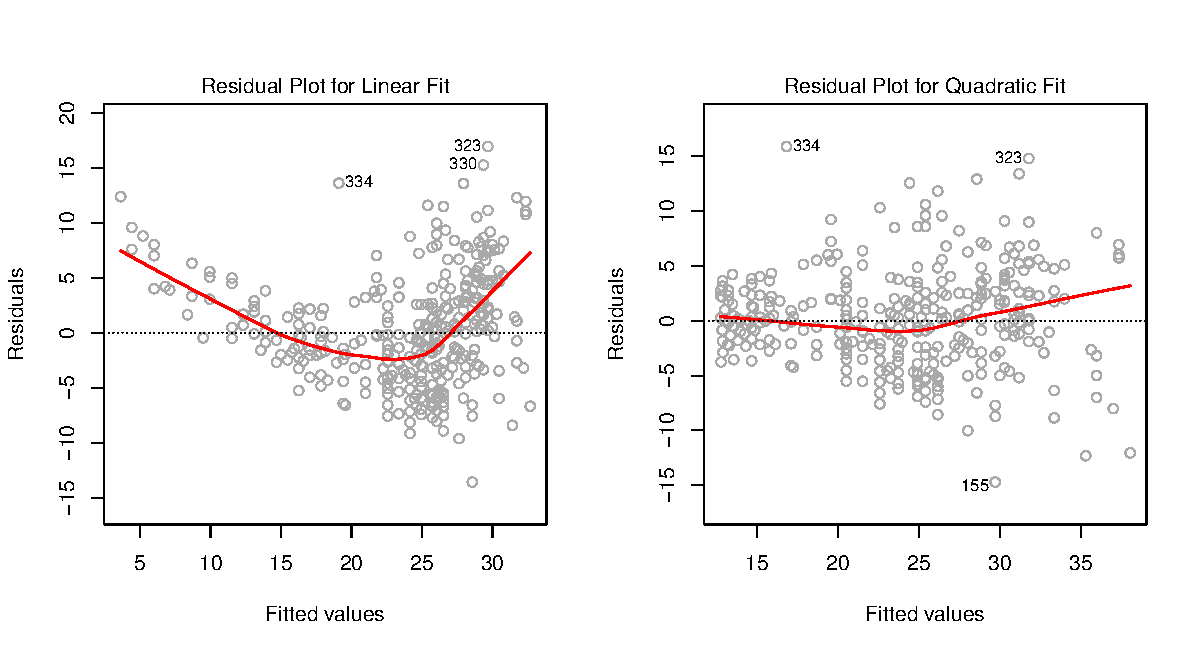
\includegraphics[width=0.85\textwidth,height=0.55\textheight,keepaspectratio]{3_9.pdf}
  \end{center}
  Left: a linear model on \texttt{mpg} vs.\ \texttt{horsepower}.
  Residuals form a clear U. Right: after adding a quadratic term ---
  the pattern is gone.
  \islpsource{Figure 3.9}
\end{frame}

% ============================================================
\begin{frame}{Exercise 3.10 --- Reading residual plots [Concept]}
  \begin{exercise}
    For each residual-vs-fitted pattern, name the problem and a remedy.
    \begin{enumerate}
      \item Residuals form a clear U-shape (curve) around zero.
      \item Residuals fan out into a funnel: small spread at low fitted
            values, large spread at high fitted values.
      \item Residuals are a random band of roughly constant width
            centred on zero.
      \item One point sits far from all others in $x$-space and pulls
            the fitted line toward it.
    \end{enumerate}
  \end{exercise}
\end{frame}

\begin{frame}{Solution --- Exercise 3.10}
  \begin{solutionbox}
    \textbf{(1) Nonlinearity.} A systematic curve means the linear
    functional form is wrong. Remedy: add polynomial terms
    ($x^2,\ldots$), transform the predictor ($\log x$, $\sqrt{x}$), or
    use a more flexible model.

    \textbf{(2) Heteroscedasticity.} The error variance grows with the
    mean --- non-constant variance. Standard errors and CIs become
    unreliable. Remedy: transform the response ($\log y$ or $\sqrt{y}$),
    use weighted least squares, or heteroscedasticity-robust
    (``sandwich'') standard errors.

    \textbf{(3) All good.} A structureless horizontal band of constant
    width is exactly what we want: the linearity, constant-variance and
    zero-mean assumptions look satisfied. No action needed.

    \textbf{(4) High-leverage point.} An extreme $x$ value has unusual
    influence on the slope. Remedy: verify it is not a data error,
    report the fit with and without it, and consider a robust
    regression. (Distinguish leverage --- unusual $x$ --- from an
    outlier --- unusual $y$; the dangerous points are high in both.)
  \end{solutionbox}
\end{frame}

\subsection{Heteroscedasticity}

\begin{frame}{Diagnostic 2: non-constant variance}
  OLS assumes $\mathrm{Var}(\varepsilon \mid X)$ is constant. When it
  isn't, the standard errors and inference become unreliable.
  \begin{block}{What to look for}
    A funnel-shaped residual plot --- the spread of residuals grows
    or shrinks systematically with the fitted value.
  \end{block}
  \begin{center}
    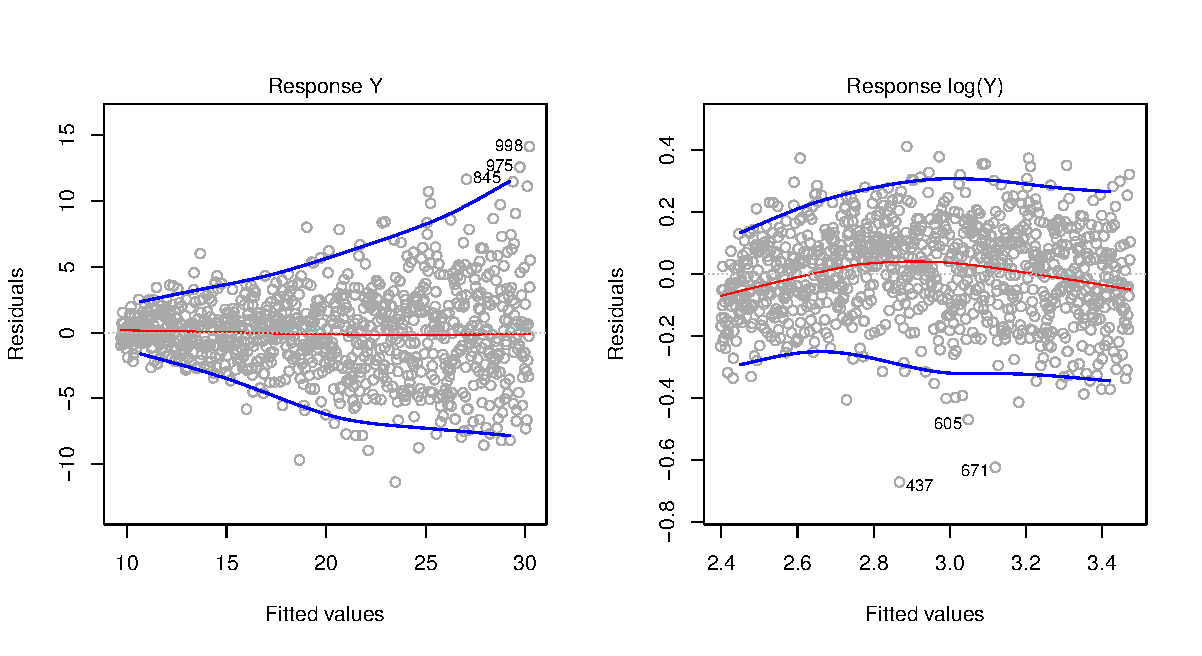
\includegraphics[width=0.78\textwidth,height=0.42\textheight,keepaspectratio]{3_11.pdf}
  \end{center}
  \islpsource{Figure 3.11}
\end{frame}

\begin{frame}{Three remedies for heteroscedasticity}
  \begin{block}{Fix the model}
    Transform the response: $\log Y$ for right-skewed positive
    responses, $\sqrt{Y}$ for count-like data. Fit OLS on the
    transformed scale.
  \end{block}
  \begin{block}{Reweight the fit}
    \emph{Weighted least squares}: give observations with smaller
    expected variance more weight, recover efficient estimates and
    valid inference.
  \end{block}
  \begin{block}{Fix the standard errors}
    Use \emph{heteroscedasticity-consistent} (sandwich / robust)
    standard errors. The point estimates are unchanged; only the SEs
    improve.
  \end{block}
\end{frame}

\subsection{Outliers and leverage}

\begin{frame}{Outlier vs.\ high-leverage: not the same thing}
  These two terms describe \emph{very different} pathologies and need
  to be diagnosed separately.
  \begin{columns}[T]
    \begin{column}{0.48\textwidth}
      \begin{block}{Outlier}
        A point with a large residual --- the model fits it badly.
        May or may not affect the fit much.
      \end{block}
    \end{column}
    \begin{column}{0.48\textwidth}
      \begin{block}{High-leverage point}
        A point with an unusual $X$ value --- it can pull the line
        strongly toward itself.
      \end{block}
    \end{column}
  \end{columns}
  \begin{alertblock}{Worst case}
    A point that is \emph{both} a high-leverage point \emph{and} an
    outlier dominates the entire fit. Always flag these.
  \end{alertblock}
\end{frame}

\begin{frame}{Detecting outliers and leverage in practice}
  Two diagnostic statistics, available in every package:
  \begin{block}{Studentised residuals}
    Each residual divided by its estimated standard deviation.
    Studentised residuals greater than $3$ in absolute value flag
    potential outliers.
  \end{block}
  \begin{block}{Leverage statistic $h_{ii}$}
    The $i$-th diagonal of the hat matrix, $h_{ii} = (\mathbf{H})_{ii}$.
    Always $0 \le h_{ii} \le 1$ with average $(p+1)/n$. Flag points with
    $h_{ii} > 2(p+1)/n$ as high-leverage.
  \end{block}
  \begin{takeaway}
    Studentised residuals catch unusual \emph{$y$}-values; leverage
    catches unusual \emph{$x$}-values. A point that trips \emph{both}
    rules is the one most likely distorting the fit.
  \end{takeaway}
\end{frame}

\begin{frame}{Outliers and leverage: visual examples}
  \begin{center}
    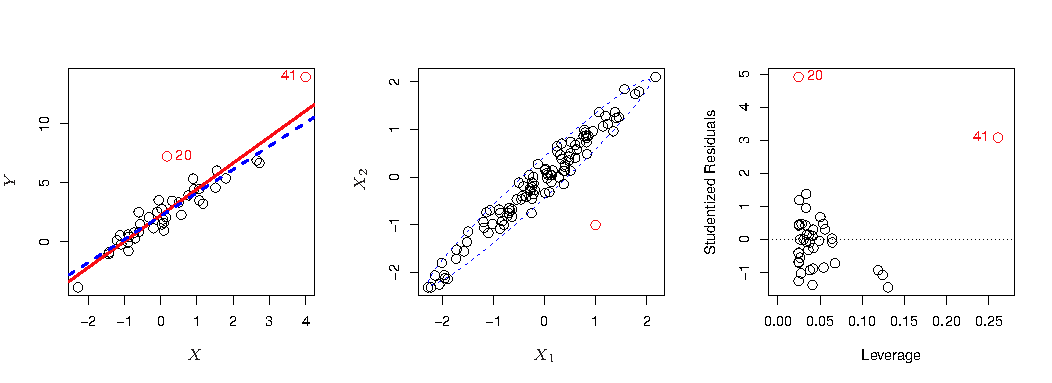
\includegraphics[width=0.85\textwidth,height=0.62\textheight,keepaspectratio]{3_13.pdf}
  \end{center}
  Left: an outlier with low leverage. Middle: a high-leverage point
  that is \emph{not} an outlier. Right: the dangerous combination.
  \islpsource{Figure 3.13}
\end{frame}

% ============================================================
\begin{frame}[fragile]{Exercise 3.11 --- Leverage and outliers [Python]}
  \begin{exercise}
    Fit $\texttt{medv}\sim\texttt{lstat}$ on the Boston data.
    \begin{enumerate}
      \item Write code to extract the leverage (hat) values and the
            studentised residuals.
      \item Flag high-leverage points using the rule
            $h_{ii} > 2(p+1)/n$ and outliers as
            $|\text{studentised residual}| > 3$.
      \item In one sentence each, explain what leverage and a
            studentised residual measure.
    \end{enumerate}
  \end{exercise}
\end{frame}

\begin{frame}[fragile]{Solution --- Exercise 3.11 (1/2)}
  \begin{solutionbox}
    \textbf{(1)--(2) Code.}
    \vspace{-2mm}
\begin{lstlisting}
import pandas as pd, numpy as np
import statsmodels.api as sm

boston = pd.read_csv("../../ALL CSV FILES - 2nd Edition/Boston.csv")
X = sm.add_constant(boston["lstat"])    # intercept + lstat
res = sm.OLS(boston["medv"], X).fit()   # fit medv ~ lstat

infl = res.get_influence()              # influence diagnostics object
lev  = infl.hat_matrix_diag             # leverage h_ii
stud = infl.resid_studentized_external  # studentized residuals

n, p = X.shape[0], X.shape[1] - 1       # n obs, p predictors
high_lev = np.where(lev > 2*(p+1)/n)[0]   # rule: h_ii > 2(p+1)/n
outliers = np.where(np.abs(stud) > 3)[0]  # rule: |stud. resid| > 3
print("high leverage:", high_lev)         # 34 tracts flagged
print("outliers:", outliers)              # 11 tracts, max |stud| = 4.0
\end{lstlisting}
  \end{solutionbox}
\end{frame}

\begin{frame}{Solution --- Exercise 3.11 (2/2)}
  \begin{solutionbox}
    \textbf{(3) Meaning.}
    \begin{itemize}
      \item \emph{Leverage} $h_{ii}$ measures how unusual an
            observation's \emph{predictor} values are; high-leverage
            points can strongly influence the fitted line. The average
            leverage is $(p+1)/n$, hence the $2(p+1)/n$ threshold.
      \item A \emph{studentised residual} is the residual divided by its
            estimated standard deviation (with that point left out); it
            flags observations with unusual \emph{response} values
            (outliers) on a comparable scale. Points that are both high
            leverage \emph{and} outliers are the most influential.
    \end{itemize}

    \textbf{What the run shows (Boston).} With $n=506$, $p=1$ the
    leverage cut-off is $2(p+1)/n=4/506\approx 0.008$, and $34$ tracts
    exceed it --- exactly the largest-\texttt{lstat} neighbourhoods.
    Eleven studentised residuals exceed $+3$ (max $\approx 4.0$): all
    are expensive tracts, mostly at the censored top value
    $\texttt{medv}=50$, which the line under-predicts. The two sets do
    not overlap here --- leverage and outlyingness really are different
    things.

    \medskip
    \textit{Common mistake:} treating the thresholds as deletion rules.
    Flagged points call for \emph{inspection} (data error? capped
    response?) and a with/without sensitivity refit --- not automatic
    removal.
  \end{solutionbox}
\end{frame}

\subsection{Collinearity}

\begin{frame}{Diagnostic 4: collinearity}
  \begin{block}{Definition}
    Two or more predictors are highly correlated, so that one is well
    approximated by a linear combination of the others.
  \end{block}
  \begin{takeaway}[Why it matters]
    The estimates $\hat\beta_j$ become unstable. Inflated standard
    errors, unstable signs, and counterintuitive coefficients are all
    classical symptoms.
  \end{takeaway}
  Curiously, predictions are usually fine; only the inferential
  interpretation of individual coefficients is corrupted.
\end{frame}

\begin{frame}{Collinearity, seen: two predictors that move together}
  \begin{center}
    
\includegraphics[width=0.92\textwidth,height=0.48\textheight,keepaspectratio]{ch03_x_collinearity.png}
  \end{center}
  \begin{takeaway}
    When two predictors nearly fall on a line (left, $r=0.997$), the data
    cannot separate their individual effects, so each coefficient swings
    wildly from sample to sample. Uncorrelated predictors (right) carry
    independent information and cause no such trouble.
  \end{takeaway}
\end{frame}

\begin{frame}{Variance inflation factor (VIF)}
  Quantify collinearity for predictor $X_j$ via:
  \begin{block}{VIF}
    \[
      \mathrm{VIF}(\hat\beta_j) = \frac{1}{1 - R^2_{X_j \mid X_{-j}}},
    \]
    where $R^2_{X_j \mid X_{-j}}$ comes from regressing $X_j$ on all the
    \emph{other} predictors. If they already explain $X_j$ almost
    perfectly, $R^2_{X_j \mid X_{-j}}\to 1$, the denominator $\to 0$, and
    $\mathrm{VIF}\to\infty$.
  \end{block}
  \begin{readme}
    \begin{itemize}
      \item $\mathrm{VIF} = 1$: no collinearity.
      \item $\mathrm{VIF} > 5$ (some authors use $10$): problematic.
      \item Remedies: drop a predictor, combine into an index, or use
            ridge regression (Ch.~6) which is robust to collinearity.
    \end{itemize}
  \end{readme}
\end{frame}


% ============================================================
\begin{frame}[fragile]{Exercise 3.12 --- Collinearity and VIF [Python]}
  \begin{exercise}
    On the Credit data, \texttt{limit} and \texttt{rating} are almost
    perfectly correlated.
    \begin{enumerate}
      \item Write code to compute the variance inflation factor (VIF)
            for the predictors \texttt{limit}, \texttt{rating} and
            \texttt{age} in a regression of \texttt{balance}.
      \item You obtain roughly $\mathrm{VIF}(\texttt{limit})\approx 160$,
            $\mathrm{VIF}(\texttt{rating})\approx 161$,
            $\mathrm{VIF}(\texttt{age})\approx 1.0$. What does VIF
            measure, and what is the consequence of these large values?
      \item Suggest two fixes.
    \end{enumerate}
  \end{exercise}
\end{frame}

\begin{frame}[fragile]{Solution --- Exercise 3.12 (1/2)}
  \begin{solutionbox}
    \textbf{(1) Code.}
\begin{lstlisting}
import pandas as pd
import statsmodels.api as sm
from statsmodels.stats.outliers_influence \
    import variance_inflation_factor as vif_

credit = pd.read_csv("../../ALL CSV FILES - 2nd Edition/Credit.csv")
cols = ["Limit", "Rating", "Age"]   # CSV column names are capitalised
X = sm.add_constant(credit[cols])   # design matrix + intercept column
# VIF_j = 1/(1 - R2 of X_j regressed on the other columns)
vifs = {col: vif_(X.values, i) for i, col in enumerate(X.columns)}
print(vifs)   # Limit ~ 160, Rating ~ 161, Age ~ 1.0
\end{lstlisting}
  \end{solutionbox}
\end{frame}

\begin{frame}{Solution --- Exercise 3.12 (2/2)}
  \begin{solutionbox}
    \textbf{(2) What VIF measures.}
    \[
      \mathrm{VIF}(\hat\beta_j)=\frac{1}{1-R_j^2},
    \]
    where $R_j^2$ is from regressing predictor $j$ on all the others. It
    is the factor by which the \emph{variance} of $\hat\beta_j$ is
    inflated because of collinearity. $\mathrm{VIF}=1$ means no
    collinearity; values above $\sim5$--$10$ are concerning. Here
    $\mathrm{VIF}\approx 160$ means the standard errors of the
    \texttt{limit} and \texttt{rating} coefficients are about
    $\sqrt{160}\approx 13$ times larger than they would be if the two
    were uncorrelated. Consequence: hugely inflated standard errors,
    unstable and possibly wrong-signed coefficients, and low power to
    detect either effect --- even though \emph{jointly} they predict
    balance well.

    \textbf{(3) Fixes.}
    \begin{itemize}
      \item Drop one of the redundant predictors (keep \texttt{limit}
            \emph{or} \texttt{rating}), since they carry nearly the same
            information.
      \item Combine them into a single index (e.g.\ an average or a
            principal component), or use a penalised method such as
            ridge regression that tolerates collinearity.
    \end{itemize}
  \end{solutionbox}
\end{frame}

% ---------------- Extended Exercise 3.L5 [Integrative] ----------------
\begin{frame}{Extended Exercise 3.L5 --- A diagnostics case study [Integrative]}
  \begin{longexercise}
    You regress house \texttt{price} on \texttt{size}, \texttt{bedrooms},
    \texttt{age} and \texttt{income} ($n=400$) and inspect the standard
    diagnostic plots:
    \begin{itemize}
      \item \textbf{Residuals vs fitted:} a clear $\cup$-shaped curve, and
            the spread of residuals \emph{widens} from left to right.
      \item \textbf{Scale--location:} $\sqrt{|\text{standardised resid}|}$
            trends steadily upward.
      \item \textbf{Residuals vs leverage:} two points with
            $|\text{studentised resid}|>3$; one point on the far right with
            leverage $h_{ii}=0.30$ (average $\bar h=5/400=0.0125$) and a
            large Cook's distance.
      \item \textbf{VIF:} size $8.9$, bedrooms $7.5$, age $1.3$, income $9.2$.
    \end{itemize}
    Diagnose \emph{all four} classical problems and recommend a concrete
    fix for each.
  \end{longexercise}
\end{frame}

\begin{frame}{Solution --- Extended Exercise 3.L5 (1/2)}
  \begin{solutionbox}
    \textbf{Nonlinearity.} A $\cup$-shaped residuals-vs-fitted plot is
    the signature of a \emph{misspecified mean} --- a straight model on a
    curved relationship. \emph{Fix:} add polynomial terms (e.g.\
    $\texttt{size}^2$) or transform a predictor ($\log\texttt{size}$);
    consider splines. Re-check for a flat, patternless band.

    \textbf{Heteroscedasticity.} Widening residuals together with an
    upward scale--location trend indicate non-constant error variance, so
    the usual SEs and the $t$-/$F$-tests are unreliable. \emph{Fix:}
    transform the response ($\log$ or $\sqrt{\ \ }$ of \texttt{price}), use
    weighted least squares, or report heteroscedasticity-robust
    (White / HC) standard errors.
  \end{solutionbox}
\end{frame}

\begin{frame}{Solution --- Extended Exercise 3.L5 (2/2)}
  \begin{solutionbox}
    \textbf{Outliers.} The two points with $|\text{studentised resid}|>3$
    are badly fit in the $y$-direction; they inflate RSE and can distort
    tests. \emph{Fix:} check for data-entry errors; report the fit with
    and without them; consider robust regression --- do \emph{not} delete
    solely because a point is large.

    \textbf{High leverage / influence.} The point with $h_{ii}=0.30$
    ($24\times$ the average $0.0125$) plus a large Cook's distance is
    unusual in $x$ \emph{and} actually moves the fit. \emph{Fix:} inspect
    it and test sensitivity by refitting without it.

    \textbf{Collinearity.} VIFs of $8.9$, $7.5$, $9.2$ (all $\gg 5$) show
    \texttt{size}, \texttt{bedrooms} and \texttt{income} carry overlapping
    information, inflating their SEs. \emph{Fix:} drop or combine a
    redundant predictor (e.g.\ keep size, or use price-per-size), or use
    ridge / PCA regression; recompute VIFs until all $<5$.
  \end{solutionbox}
\end{frame}

% ============================================================
\section{vs.\ KNN}
% ============================================================

\begin{frame}{Linear regression vs.\ KNN regression}
  KNN regression is the simplest nonparametric alternative: predict
  $Y$ at $x_0$ as the average of the $K$ nearest neighbours' responses.
  \begin{columns}[T]
    \begin{column}{0.48\textwidth}
      \textbf{Linear regression}
      \begin{itemize}
        \item Assumes a global functional form.
        \item Few parameters $\Rightarrow$ low variance.
        \item Interpretable coefficients.
      \end{itemize}
    \end{column}
    \begin{column}{0.48\textwidth}
      \textbf{KNN regression}
      \begin{itemize}
        \item No functional form.
        \item Many ``effective'' parameters $\Rightarrow$ low bias if
              $f$ is nonlinear.
        \item Hard to interpret.
      \end{itemize}
    \end{column}
  \end{columns}
  \begin{takeaway}
    Rule of thumb: with few observations, many predictors, or a roughly
    linear truth, prefer regression. KNN wins only when the truth is
    strongly nonlinear \emph{and} $n$ is large enough to fill the space.
  \end{takeaway}
\end{frame}

\begin{frame}{Linear vs.\ KNN: simulation}
  \begin{center}
    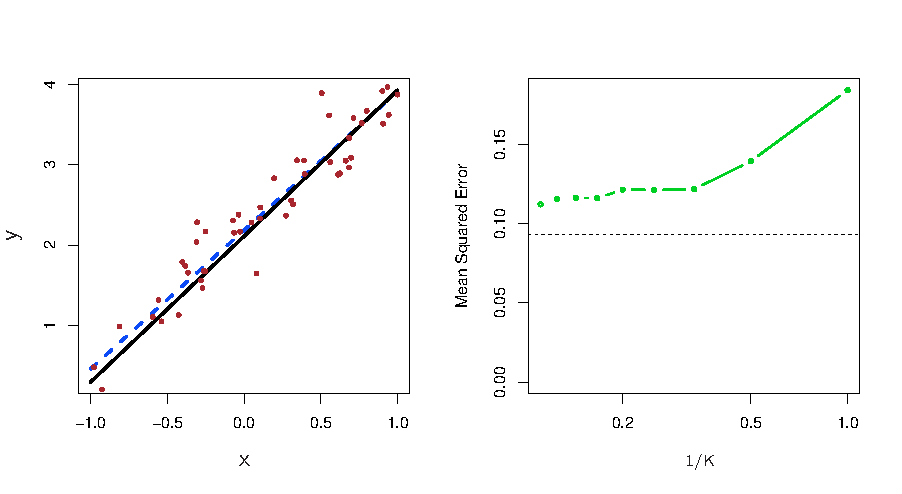
\includegraphics[width=0.85\textwidth,height=0.66\textheight,keepaspectratio]{3_18.pdf}
  \end{center}
  When the truth is approximately linear (left), linear regression
  dominates KNN. When the truth is highly nonlinear (right), KNN
  wins --- if $n$ is large enough.
  \islpsource{Figure 3.18}
\end{frame}

\begin{frame}{The curse of dimensionality strikes KNN}
  \begin{center}
    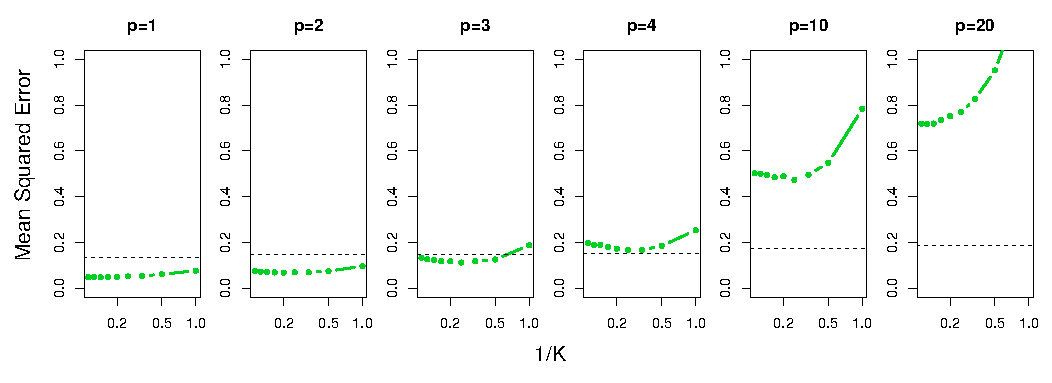
\includegraphics[width=0.82\textwidth,height=0.55\textheight,keepaspectratio]{3_20.pdf}
  \end{center}
  As $p$ grows, KNN performance deteriorates rapidly: in high
  dimensions there are no truly ``near'' neighbours. Linear methods
  are more robust because they impose structure.
  \islpsource{Figure 3.20}
\end{frame}


% ---------------- Extended Exercise 3.L6 [Python] ----------------
\begin{frame}[fragile]{Extended Exercise 3.L6 --- Linear vs polynomial vs KNN [Python]}
  \begin{longexercise}
    On \texttt{Auto.csv}, model $\texttt{mpg}\sim\texttt{horsepower}$
    (drop the rows where \texttt{horsepower} is the string \texttt{"?"}).
    \begin{enumerate}
      \item Make a $70/30$ split (\texttt{random\_state=1}) and fit three
            models: linear, degree-2 polynomial, and KNN regression
            (standardise $x$ first).
      \item Estimate the \emph{test} MSE of each.
      \item Which fits best, and why? Answer in terms of the
            \emph{bias--variance trade-off}, and say what happens to KNN as
            $K\to 1$.
    \end{enumerate}
  \end{longexercise}
\end{frame}

\begin{frame}[fragile]{Solution --- Extended Exercise 3.L6 (1/3)}
  \begin{solutionbox}
    \textbf{Load, clean and split.}
\begin{lstlisting}[basicstyle=\ttfamily\scriptsize]
import pandas as pd
from sklearn.model_selection import train_test_split
from sklearn.linear_model import LinearRegression
from sklearn.preprocessing import PolynomialFeatures, StandardScaler
from sklearn.pipeline import make_pipeline
from sklearn.neighbors import KNeighborsRegressor
from sklearn.metrics import mean_squared_error as mse   # test-error metric

a = pd.read_csv("../../ALL CSV FILES - 2nd Edition/Auto.csv")  # load Auto data
a = a[a.horsepower != "?"]; a.horsepower = a.horsepower.astype(float)  # clean
X, y = a[["horsepower"]].values, a["mpg"].values  # one predictor, target mpg
Xtr, Xte, ytr, yte = train_test_split(X, y, test_size=.3, random_state=1)  # 70/30
\end{lstlisting}
  \end{solutionbox}
\end{frame}

\begin{frame}[fragile]{Solution --- Extended Exercise 3.L6 (2/3)}
  \begin{solutionbox}
    \textbf{Fit the three models and score the test MSE.}
\begin{lstlisting}[basicstyle=\ttfamily\scriptsize]
lin = LinearRegression().fit(Xtr, ytr)                    # straight-line fit
pol = make_pipeline(PolynomialFeatures(2), LinearRegression()).fit(Xtr, ytr)  # adds hp^2
knn = make_pipeline(StandardScaler(), KNeighborsRegressor(10)).fit(Xtr, ytr)  # scale, K=10
for name, m in [("linear", lin), ("poly-2", pol), ("KNN10", knn)]:
    print(name, round(mse(yte, m.predict(Xte)), 1))       # test-set MSE
# linear 26.2 | poly-2 19.8 | KNN(K=10) 21.3
\end{lstlisting}
  \end{solutionbox}
\end{frame}

\begin{frame}{Solution --- Extended Exercise 3.L6 (3/3)}
  \begin{solutionbox}
    \textbf{Test MSE.} Linear $\approx 26.2$, degree-2 polynomial
    $\approx 19.8$, KNN $(K{=}10)\approx 21.3$: both flexible models
    clearly beat the straight line.

    \textbf{Why (bias--variance).} The true \texttt{mpg}--\texttt{horsepower}
    relationship is convex and decreasing, so a straight line
    \emph{underfits} --- high \emph{bias}, largest test MSE. The degree-2
    polynomial captures the curvature with just one extra parameter (low
    bias, still low variance) and wins here; a moderate-$K$ KNN is a close
    non-parametric competitor.

    \textbf{As $K\to 1$.} Each prediction is a single neighbour: the model
    interpolates the training points (training MSE $\to 0$) but is very
    wiggly --- high \emph{variance}, so test MSE \emph{rises} (here
    $\approx 34$ at $K{=}1$). The best $K$ balances bias (large $K$)
    against variance (small $K$). \emph{Takeaway:} prefer the parsimonious
    degree-2 fit; if using KNN, tune $K$ by cross-validation.
  \end{solutionbox}
\end{frame}

% ============================================================
\section{Python Lab}

\begin{frame}{Python lab --- run it live in the notebook}
  \begin{labnote}[Companion notebook: \texttt{chapter\_03\_lab.ipynb}]
    The code in this section is meant to be \textbf{demonstrated live}. Open the companion Jupyter notebook and run it cell by cell:
    \begin{itemize}
      \item simple and multiple linear regression with \texttt{statsmodels};
      \item polynomials and interactions via the ISLP \texttt{ModelSpec};
      \item regression diagnostics; and a comparison with KNN.
    \end{itemize}
    Data loads via the \texttt{ISLP} package or the bundled CSV files; the notebook ends with hands-on exercises.
  \end{labnote}
\end{frame}


% ============================================================

\begin{frame}[fragile]{Simple regression with statsmodels}
  \begin{lstlisting}
import pandas as pd, numpy as np
import statsmodels.api as sm
from ISLP import load_data             # textbook data sets

Boston = load_data("Boston")           # Boston housing data
X = sm.add_constant(Boston["lstat"])   # predictor + intercept column
y = Boston["medv"]                     # response: median home value
res = sm.OLS(y, X).fit()               # least-squares fit medv ~ lstat
print(res.summary())                   # coef, SE, t, p, CI, R2, F
  \end{lstlisting}
  \texttt{statsmodels} produces a comprehensive output table with
  coefficients, standard errors, $t$-statistics, $p$-values, and
  confidence intervals --- everything we need for inference.
\end{frame}

\begin{frame}[fragile]{Confidence and prediction intervals}
  \begin{lstlisting}
xnew = pd.DataFrame({"const": 1.0, "lstat": [5, 10, 15]})  # new x
pred = res.get_prediction(xnew)   # predictions with uncertainty
pred.summary_frame(alpha=0.05)    # 95% intervals of both kinds
# columns: mean, mean_se,
#   mean_ci_lower / upper,        <- CI
#   obs_ci_lower  / upper         <- prediction interval
  \end{lstlisting}
  Both intervals come from the same fit but answer different
  questions. Always use \emph{prediction} intervals when communicating
  uncertainty about an individual outcome.
\end{frame}

\begin{frame}[fragile]{Multiple regression}
  \begin{lstlisting}
predictors = ["lstat", "age", "rm", "ptratio", "tax"]  # five inputs
X = sm.add_constant(Boston[predictors])  # design matrix + intercept
res = sm.OLS(Boston["medv"], X).fit()    # fit multiple regression
print(res.summary())                     # one t-test per coefficient
  \end{lstlisting}
  Adding more predictors typically increases $R^2$ and shrinks the
  per-coefficient standard errors --- as long as the new variables are
  not collinear.
\end{frame}

\begin{frame}[fragile]{Polynomials and interactions via ISLP}
  \begin{lstlisting}
from ISLP.models import ModelSpec as MS, poly

terms = [poly("lstat", degree=2), "age",   # lstat + lstat^2, age
         ("lstat", "age")]                 # tuple = interaction term
design = MS(terms).fit_transform(Boston)   # build the design matrix
res2 = sm.OLS(Boston["medv"], design).fit()  # then fit as usual
print(res2.summary())
  \end{lstlisting}
  \texttt{ModelSpec} produces a \texttt{statsmodels}-ready design
  matrix and handles dummies, interactions, polynomials, and splines
  cleanly.
\end{frame}

\begin{frame}[fragile]{Diagnostic plots}
  \begin{lstlisting}
import matplotlib.pyplot as plt
fig, axes = plt.subplots(1, 2, figsize=(10, 4))    # two panels
axes[0].scatter(res.fittedvalues, res.resid, s=8)  # resid vs fitted
axes[0].axhline(0, color="grey", linewidth=0.8)    # zero line
axes[0].set_xlabel("Fitted"); axes[0].set_ylabel("Residual")
sm.qqplot(res.resid, line="45", ax=axes[1])        # normality check
plt.tight_layout(); plt.show()                     # render figure
  \end{lstlisting}
  Two diagnostic plots that should be made for every regression: the
  residual-vs.-fitted plot and the Q-Q plot.
\end{frame}

\begin{frame}[fragile]{Leverage and VIF}
  \begin{lstlisting}
from statsmodels.stats.outliers_influence \
    import variance_inflation_factor as vif_

infl = res.get_influence()   # influence diagnostics object
lev = infl.hat_matrix_diag   # leverage values h_ii
high_lev = np.where(lev > 2*X.shape[1]/X.shape[0])[0]  # h > 2(p+1)/n

vifs = [vif_(X.values, j) for j in range(X.shape[1])]  # VIF per column
print(dict(zip(X.columns, vifs)))  # VIF near 1 fine; > 5 problematic
  \end{lstlisting}
  Always inspect leverage and VIF before declaring an analysis
  complete.
\end{frame}


% ============================================================
\section{Summary}
% ============================================================

\begin{frame}{Chapter 3 in one slide}
  \begin{block}{What we accomplished}
    Built up linear regression from one predictor to many, with full
    inferential machinery and diagnostics.
  \end{block}
  \begin{itemize}
    \item Estimated $\beta$ by least squares; derived standard errors,
          $t$- and $F$-tests.
    \item Saw how multiple regression handles confounding.
    \item Encoded qualitative predictors and added interaction terms.
    \item Diagnosed nonlinearity, heteroscedasticity, outliers,
          leverage, and collinearity.
    \item Compared linear regression with KNN regression.
  \end{itemize}
\end{frame}

\begin{frame}{Vocabulary checklist}
  \footnotesize
  \begin{tabular}{ll}
    \toprule
    \textbf{Term} & \textbf{Meaning} \\
    \midrule
    SLR / MLR & Simple / multiple linear regression \\
    OLS & Ordinary least squares \\
    RSS / TSS / RSE & Residual / total sum of squares; $\sqrt{\mathrm{RSS}/(n-p-1)}$ \\
    $R^2$ / adj.\ $R^2$ & Variance explained / penalised version \\
    $t$-test / $F$-test & One $\beta_j$ / all $\beta_j$ at once \\
    Confidence vs.\ prediction interval & On the line / on a future $Y$ \\
    Hat matrix $\mathbf{H}$ & $\mathbf{X}(\mathbf{X}^\top\mathbf{X})^{-1}\mathbf{X}^\top$ \\
    Leverage $h_{ii}$ & Diagonal of $\mathbf{H}$; flag if $> 2(p+1)/n$ \\
    Studentised residual & Residual divided by its estimated SD \\
    VIF & $1/(1 - R^2_{X_j \mid X_{-j}})$ \\
    Interaction & Effect of $X_1$ depends on $X_2$ \\
    \bottomrule
  \end{tabular}
\end{frame}

\begin{frame}{Key formulas at a glance}
  \begin{block}{OLS estimates}
    \[
      \hat\beta_1 = \frac{\sum (x_i - \bar x)(y_i - \bar y)}
                         {\sum (x_i - \bar x)^2},
      \qquad
      \hat\beta_0 = \bar y - \hat\beta_1 \bar x,
      \qquad
      \hat{\boldsymbol\beta} = (\mathbf{X}^\top\mathbf{X})^{-1}\mathbf{X}^\top\mathbf{y}.
    \]
  \end{block}
  \begin{block}{Tests}
    \[
      t_j = \frac{\hat\beta_j}{\mathrm{SE}(\hat\beta_j)} \sim t_{n-p-1},
      \qquad
      F = \frac{(\mathrm{TSS} - \mathrm{RSS})/p}
              {\mathrm{RSS}/(n - p - 1)} \sim F_{p,\,n-p-1}.
    \]
  \end{block}
\end{frame}

\begin{frame}{Decision rules of thumb}
  \begin{block}{Always}
    Plot residuals vs.\ fitted values. Plot residuals vs.\ each
    predictor. Compute VIFs. Examine high-leverage observations.
  \end{block}
  \begin{block}{Rules of thumb}
    \begin{itemize}
      \item $|t_j| > 2$ or $p < 0.05$ $\Rightarrow$ ``statistically
            significant'' --- but always also check effect size.
      \item $\mathrm{VIF} > 5$ (some say $10$) $\Rightarrow$ collinearity
            worth addressing.
      \item Funnel-shape residuals $\Rightarrow$ try a log transformation
            or robust SEs.
      \item Curved residual mean $\Rightarrow$ add polynomial / spline.
    \end{itemize}
  \end{block}
\end{frame}

\begin{frame}{Common pitfalls}
  \begin{alertblock}{Don't}
    \begin{enumerate}
      \item Interpret a univariate slope as a causal effect.
      \item Trust $p$-values when residuals are obviously non-normal or
            heteroscedastic.
      \item Add an interaction without keeping the main effects
            (hierarchy principle).
      \item Use stepwise selection with naive $p$-values --- the
            standard errors are wrong.
      \item Report only $R^2$ on training data without out-of-sample
            checks.
      \item Forget to check leverage --- a few points can dominate the
            entire fit.
    \end{enumerate}
  \end{alertblock}
\end{frame}

\begin{frame}{Self-check questions}
  \begin{enumerate}
    \item Derive the OLS slope $\hat\beta_1$ from the normal equations.
    \item Why does adding any predictor never decrease $R^2$? What is
          the fix?
    \item Suppose two predictors are perfectly correlated. What goes
          wrong with OLS? With ridge?
    \item Interpret an interaction coefficient
          $\beta_3\,X_1 X_2 = 0.4$ when $X_1$ = TV spend in \$1k and
          $X_2$ = radio spend in \$1k.
    \item In the Boston data, the simple regression of \texttt{medv}
          on \texttt{age} is significantly negative, but in the
          multiple regression it is not. Explain.
    \item State the prediction interval for a new observation at $x_0$
          and contrast with the confidence interval.
  \end{enumerate}
\end{frame}

\begin{frame}{Ten things to remember}
  \begin{enumerate}
    \item Linear regression: linear in the coefficients, not in $X$.
    \item Least squares minimises the squared residuals.
    \item Standard errors $\to$ confidence intervals and $t$-tests.
    \item $F$-test answers ``is any predictor useful?''.
    \item Each $\beta_j$ holds the others fixed (interpretation rule).
    \item Univariate slopes can mislead --- multiple regression matters.
    \item Encode categories as dummies; consider interactions.
    \item Diagnose: nonlinearity, heteroscedasticity, outliers,
          leverage, collinearity.
    \item Confidence vs.\ prediction intervals: line vs.\ point.
    \item Linear regression is hard to beat on small/medium tabular
          data.
  \end{enumerate}
\end{frame}

\begin{frame}{What's next}
  Chapter 4: \emph{Classification}.
  \begin{itemize}
    \item Logistic regression as the linear model for log-odds.
    \item Discriminant analysis (LDA, QDA, naive Bayes).
    \item Confusion matrices, ROC curves, AUC.
    \item Generalised linear models in one frame.
  \end{itemize}
\end{frame}

\end{document}
